\chapter{Efficiency}
\label{sec:RKst_efficiency}

The efficiency for each of the decay channels is calculated according to the formula
\begin{equation}
\varepsilon^{tot}=\varepsilon(geom)\varepsilon(reco|geom)\varepsilon(PID|reco)\varepsilon(trig|PID)\varepsilon(MVA|trig).
\end{equation}
In this expression the first term is the efficiency to have final state particles in the LHCb detector 
acceptance. The second term carries information on reconstruction and stripping efficiency
(we keep these together given that boundaries between them are completely artificial).
The third part corresponds to the efficiency of the PID requirements.
The fourth term handles the trigger efficiency for those events which are selected by the preselection process.
Finally, the latter term deals with the efficiency of the NN classifier.
Reconstruction, trigger and MVA efficiencies are evaluated on simulated data with the trigger efficiency
for $\Bz\to\Kstar\jpsi$ being cross-checked using the data-driven TISTOS method as described in Sec.~\ref{sec:Lb_trigger_eff}.
The PID efficiency is calculated with a data-driven method as described in Sec.~\ref{sec:RKst_pid_eff}.

All absolute efficiencies for the muon and electron rare channels are separately listed in Tab.~\ref{tab:RKst_AbsEff}
for the central and high \qsq intervals and in Tab.~\ref{tab:AbsEff_jpsi} for the resonant channels.
However for the analysis itself only efficiencies relative to the resonant channels are used in order
to limit systematic uncertainties.
%($\varepsilon(\Bz\to\Kstar ee)/\varepsilon(\Bz\to\Kstar(\jpsi\to ee))$)/($\varepsilon(\Bz\to\Kstar \mumu)/\varepsilon(\Bz\to\Kstar(\jpsi\to \mumu))$).
%Systematic uncertainties for relative efficiencies take into account that some effects are correlated between two decays.
%In table \ref{tab:AbsEffs} are reported absolute efficiencies
%for the electron and muon channels in the \qsq bin $1 < q^2 < 6$ \gevgevcccc.

Tab.~\ref{tab:RKst_AbsEff} reports relative efficiencies between the rare and resonant channels,
$\varepsilon(\Bz\to\Kstarz \ll)/\varepsilon(\Bz\to\Kstarz(\jpsi\to \ll))$.
Finally, in Tab.~\ref{tab:double_rel_eff} are listed ratios of relative efficiencies
for the $ee$ and $\mu\mu$ channels, $[ee/(\jpsi \to ee)] / [\mu\mu/(\jpsi\to \mu\mu)]$.
%In particular the latter table contains the total double-relative
%efficiency, $\varepsilon_tot^{drel} = \pm $, which is used for the final result extraction.

\begin{table}[h!]
\centering
\caption{Absolute efficiencies for the resonant $ee$ and $\mu\mu$ channels.}
\begin{tabular}{|c|c|c|c|c|}
\hline \multirow{2}{*}{$\varepsilon$} 	&  $\mu\mu$ 	& \multicolumn {3}{c|}{$ee$} \\ \cline{2-5}
	  & &  L0E 	& L0H 	& L0I \\ \hline
Geom  & $ 0.1598  \pm  0.0005 $ & \multicolumn{3}{c|}{$ 0.1589  \pm  0.0005 $} \\
Reco  & $ 0.0947  \pm  0.0001 $ & \multicolumn{3}{c|}{$ 0.0603  \pm  0.0001 $} \\
PID  & $ 0.8148  \pm  0.0000 $ & \multicolumn{3}{c|}{$ 0.8222  \pm  0.0000 $} \\
\hline
Trig  & $ 0.7620  \pm  0.0005 $ & $ 0.1976  \pm  0.0005 $ & $ 0.0166  \pm  0.0002 $ & $ 0.0720  \pm  0.0003 $ \\
MVA  & $ 0.8958  \pm  0.0004 $ & $ 0.8586  \pm  0.0007 $ & $ 0.8974  \pm  0.0006 $ & $ 0.8260  \pm  0.0017 $ \\
\hline
Tot  & $ 0.0084  \pm  0.0000 $ & $ 0.0013  \pm  0.0000 $ & $ 0.0001  \pm  0.0000 $ & $ 0.0005  \pm  0.0000 $ \\
\hline
\end{tabular}
\label{tab:AbsEff_jpsi}
\end{table}

\begin{table}[h!]
\centering
\caption{Double ratios of efficiencies 
$(\varepsilon^{ee} / \varepsilon^{\jpsi\to ee}) / (\varepsilon^{\mumu} / \varepsilon^{\jpsi\to\mumu})$
in the central and high \qsq intervals.}
\begin{tabular}{|c|c|c|c|c|}
\hline
\multirow{2}{*}{$\varepsilon$}  &  \multicolumn{3}{c|}{ 1--6~\gevgevcccc} &  \multicolumn{1}{c|}{ 15--20~\gevgevcccc } \\
\cline{2-5} &   L0E 	& L0H 	& L0I &  L0E 	\\ \hline
$q^2$  & \multicolumn{3}{c|}{$ 0.697 \pm 0.007 $} &  \multicolumn{1}{c|}{$ 0.770 \pm 0.010 $} \\
Geom  & \multicolumn{3}{c|}{$ 1.022 \pm 0.012 $} &  \multicolumn{1}{c|}{$ 1.022 \pm 0.012 $} \\
Reco  & \multicolumn{3}{c|}{$ 0.931 \pm 0.006 $} &  \multicolumn{1}{c|}{$ 0.443 \pm 0.443 $} \\
PID  & \multicolumn{3}{c|}{$ 0.982 \pm 0.000 $} &  \multicolumn{1}{c|}{$ 0.970 \pm 0.000 $} \\
\hline
Trig  & $ 0.890 \pm 0.008 $ & $ 2.449 \pm 0.049 $ & $ 1.239 \pm 0.016 $ & $ 1.416 \pm 0.014 $  \\ 
MVA  & $ 0.969 \pm 0.003 $ & $ 0.941 \pm 0.003 $ & $ 0.972 \pm 0.006 $ & $ 1.061 \pm 0.006 $  \\  
\hline
Tot  & $ 1.155 \pm 0.023 $ & $ 3.086 \pm 0.083 $ & $ 1.613 \pm 0.037 $ & $ 0.856 \pm 0.020 $  \\  
\hline
\end{tabular}
\label{tab:double_rel_eff}
\end{table}

\begin{landscape}

\begin{table}
\centering
\caption{Absolute efficiencies for the rare $ee$ and $\mu\mu$ channels in the central and high \qsq intervals.}
\begin{tabular}{|c|c|c|c|c|c|c|}
\hline \multirow{3}{*}{$\varepsilon$} 			&  \multicolumn {2}{c|}{$\mu\mu$} 				& \multicolumn {4}{c|}{$ee$} \\ \cline{2-7}
			 & 1--6~\gevgevcccc				& 15--20~\gevgevcccc  				& \multicolumn {3}{c|}{1--6~\gevgevcccc} 				& \multicolumn {1}{c|}{15--20~\gevgevcccc }\\ \cline{2-7}
				&  \multicolumn {2}{c|}{} &  L0E 	& L0H 	& L0I 	& L0E 	\\ \hline
$q^2$  & $ 0.2142  \pm  0.0015 $ & $ 0.1552  \pm  0.0013 $ &  \multicolumn{3}{c|}{$ 0.1493  \pm  0.0012 $} & \multicolumn{1}{c|}{$ 0.1196  \pm  0.0011 $} \\
Geom  & $ 0.1630  \pm  0.0014 $ & $ 0.1630  \pm  0.0014 $ &  \multicolumn{3}{c|}{$ 0.1657  \pm  0.0012 $} & \multicolumn{1}{c|}{$ 0.1657  \pm  0.0012 $} \\
Reco  & $ 0.0177  \pm  0.0001 $ & $ 0.0110  \pm  0.0001 $ &  \multicolumn{3}{c|}{$ 0.0105  \pm  0.0000 $} & \multicolumn{1}{c|}{$ 0.0031  \pm  0.0000 $} \\
PID  & $ 0.7824  \pm  0.0002 $ & $ 0.8420  \pm  0.0001 $ &  \multicolumn{3}{c|}{$ 0.7750  \pm  0.0001 $} & \multicolumn{1}{c|}{$ 0.8239  \pm  0.0001 $} \\
\hline
Trig  & $ 0.6852  \pm  0.0029 $ & $ 0.8456  \pm  0.0028 $ & $ 0.1581  \pm  0.0012 $ & $ 0.0366  \pm  0.0006 $ & $ 0.0802  \pm  0.0009 $ & $ 0.3105  \pm  0.0028 $  \\
MVA  & $ 0.9097  \pm  0.0022 $ & $ 0.8298  \pm  0.0032 $ & $ 0.8447  \pm  0.0021 $ & $ 0.8571  \pm  0.0020 $ & $ 0.8156  \pm  0.0046 $ & $ 0.8436  \pm  0.0033 $  \\
\hline
Tot  & $ 0.0066  \pm  0.0001 $ & $ 0.0068  \pm  0.0001 $ & $ 0.0012  \pm  0.0000 $ & $ 0.0003  \pm  0.0000 $ & $ 0.0006  \pm  0.0000 $ & $ 0.0009  \pm  0.0000 $  \\
\hline
\end{tabular}
\label{tab:RKst_AbsEff}
\end{table}


\begin{table}
\centering
\caption{Relative efficiencies, $\varepsilon^{rel} = \varepsilon^{\ell\ell} / \varepsilon^{\jpsi}$,
for the $ee$ and $\mu\mu$ channels in the central and high \qsq intervals.}
\begin{tabular}{|c|c|c|c|c|c|c|}
\hline \multirow{3}{*}{$\varepsilon$}  			&  \multicolumn{4}{c|}{1--6~\gevgevcccc}  				& \multicolumn {2}{c|}{15--20~\gevgevcccc}  \\ \cline{2-7}
 				&	  $\mu\mu$  				& \multicolumn {3}{c|}{$ee$} 			&  $\mu\mu$  				& \multicolumn {1}{c|}{$ee$} \\ \cline{2-7}
				&   &  L0E 	& L0H 	& L0I    &  	& L0E 	\\ \hline
Geom  & $ 1.0200 \pm 0.0091$ & \multicolumn{3}{c|}{$ 1.0429 \pm 0.0084$} & $ 1.0200 \pm 0.0091$ & \multicolumn{1}{c|}{$ 1.0429 \pm 0.0084$} \\
Reco  & $ 0.1873 \pm 0.0011$ & \multicolumn{3}{c|}{$ 0.1743 \pm 0.0006$} & $ 0.1159 \pm 0.0009$ & \multicolumn{1}{c|}{$ 0.0513 \pm 0.0003$} \\
PID  & $ 0.9602 \pm 0.0002$ & \multicolumn{3}{c|}{$ 0.9425 \pm 0.0001$} & $ 1.0334 \pm 0.0001$ & \multicolumn{1}{c|}{$ 1.0021 \pm 0.0001$} \\
\hline
Trig  & $ 0.8993 \pm 0.0038 $ & $ 0.8002 \pm 0.0065 $ & $ 2.2025 \pm 0.0434 $ & $ 1.1138 \pm 0.0136 $ & $ 1.1098 \pm 0.0037 $ & $ 1.5715 \pm 0.0145 $ \\ 
MVA  & $ 1.0154 \pm 0.0025 $ & $ 0.9838 \pm 0.0025 $ & $ 0.9551 \pm 0.0023 $ & $ 0.9874 \pm 0.0060 $ & $ 0.9262 \pm 0.0036 $ & $ 0.9825 \pm 0.0039 $ \\  
\hline
Tot  & $ 0.7821 \pm 0.0108 $ & $ 0.9033 \pm 0.0132 $ & $ 2.4136 \pm 0.0558 $ & $ 1.2618 \pm 0.0228 $ & $ 0.8092 \pm 0.0126 $ & $ 0.6923 \pm 0.0117 $ \\  
\hline
\end{tabular}\label{tab:RKst_releff}
\end{table}

\end{landscape}


\section{Geometric efficiency}


The simulated samples used contain the requirement that daughters are in the LHCb
detector acceptance. This corresponds to the requirement for each of the final particles
to have polar angle $\theta$ between 10 and 400 mrad. The efficiency of this
cuts is obtained using a generator level simulated sample.

\section{Reconstruction efficiency and bin migration}

The reconstruction efficiency is here defined as the efficiency to reconstruct
each decay channel given that its daughters are into the geometrical acceptance
of the detector. This includes both the probability that a particle generates
observable signatures and the efficiency of all the preselection cuts described in Sec.~\ref{sec:RKst_selection},
including those done to remove peaking backgrounds. 
%This efficiency is evaluated on simulated events
%to which the full list of weights described in Sec.~\ref{sec:RKst_weights} is applied.
The efficiency of the PID cuts is kept separate as it is known to be not well simulated
and there are reliable data-driven methods which can be used to extract it (see Sec.~\ref{sec:RKst_pid_eff}).

It can happen that events generated in a \qsq interval are reconstructed in a different one,
this is referred to as ``bin migration''. Two different effects can cause bin migration.
First of all, as the resolution of real detectors is not perfect, events close to the edges
of the considered intervals can fall on the wrong side of the edge. This effect is only important
in case of non-flat true distributions, as the amount of bin migration in the two directions is different.
The second possible source of bin migration are systematic effects due, for example,
to the presence of bremsstrahlung photons that cannot be recovered.
It is particularly important to take into account the bin migration in the electron channels case 
because more photons are radiated from the final state.
Figure~\ref{fig:ee_bin_mig} reports the response matrix for simulated $\decay{\Bz}{\Kstarz\ee}$ events,
which shows the correlation between reconstructed and generated \qsq. In the ideal case of
perfect resolution and no bias this plot would look like a diagonal line and in the case of no bias
its slope would be 1.
Table \ref{tab:bin_mig} reports net amounts of bin migration, $M_{net}$, in the considered \qsq intervals defined as:
%
\begin{equation}
M_{net} = N(\text{in} \to \text{in}) + N(\text{out} \to \text{in}) - N(\text{in} \to \text{out}) 
\end{equation}
%
\noindent
where $N(\text{in} \to \text{in})$ is the number of candidates that are generated and
reconstructed inside the considered interval, $N(\text{out} \to \text{in})$ the number of 
candidates that are generated outside the interval but reconstructed inside and
$N(\text{in} \to \text{out})$ the number of candidates generated inside that fall outside.

\begin{figure}[h!]
\centering
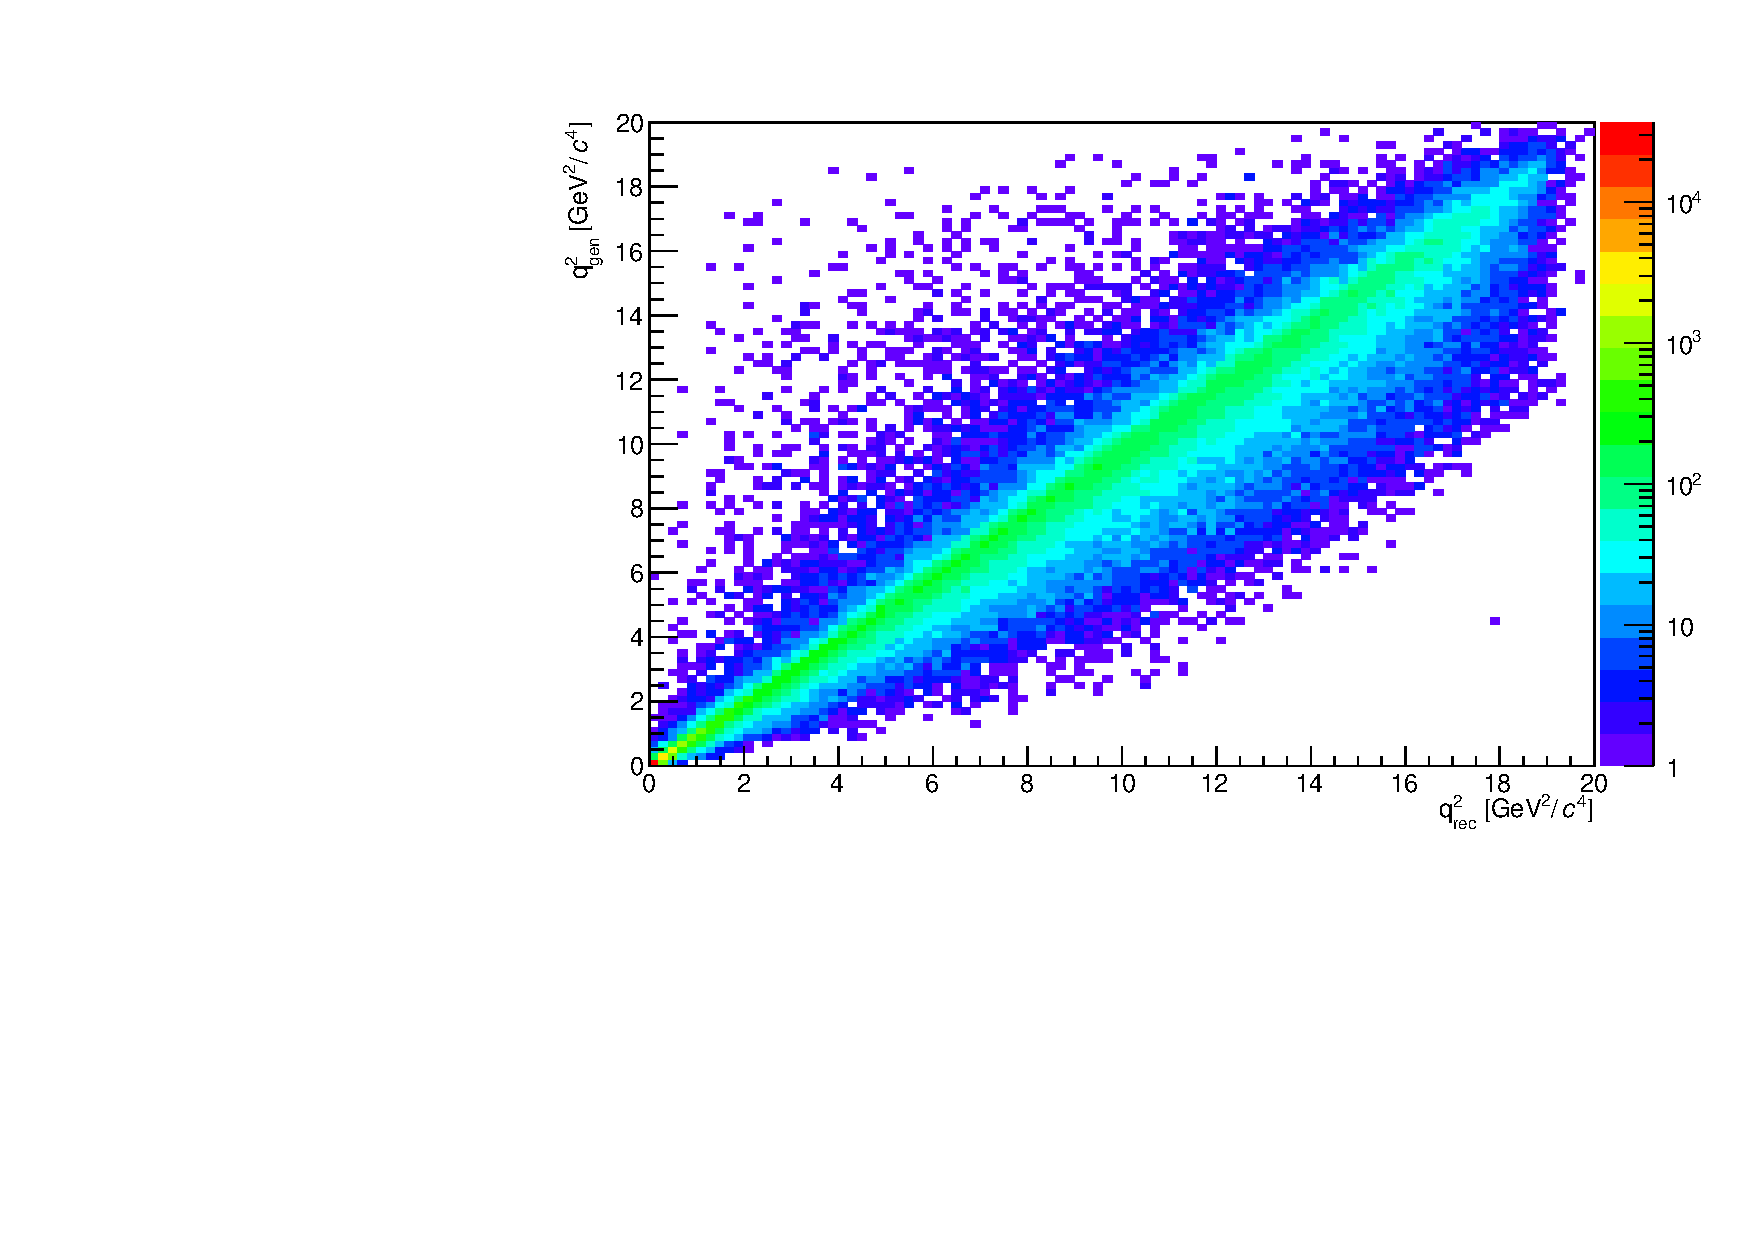
\includegraphics[width=0.85\textwidth]{RKst/figs/bin_mig.pdf}
\caption{Generated versus reconstructed \qsq in simulated $\decay{\Bz}{\Kstar ee}$ events.}
\label{fig:ee_bin_mig}
\end{figure}

\begin{table}[bh]
\centering
\caption{Net bin migration amounts ($M_{net}$) in the considered \qsq intervals.
Positive values indicate ``net in", negative values ``net out".}
\begin{tabular}{|c|c|c|c|}
\hline
 Sample 			& 1--6 GeV$^2/c^4$ 				& 15--20 GeV$^2/c^4$ 				& $J/\psi$  \\ \hline
$\mu\mu$ 	& $ -0.0018  \pm  0.0002 $ & $ 0.0042  \pm  0.0003 $ & $ -0.0012  \pm  0.0000 $ \\
$ee$ 	& $ 0.0834  \pm  0.0013 $ & $ -0.4469  \pm  0.0091 $ & $ -0.0258  \pm  0.0003 $ \\
\hline 
 \end{tabular}
 \label{tab:bin_mig}
\end{table}

The reconstruction efficiency is calculated comparing generated to reconstructed samples
and therefore already includes bin migration effects. Nevertheless, it is useful to single
out this component to better asses the corresponding systematic uncertainties.



\section{PID efficiency}
\label{sec:RKst_pid_eff}

The Monte Carlo is known not to reliably describe particle ID variables
and therefore a data-driven method is used to obtain this efficiency component.
This is done using the \verb!PIDCalib! described in Sec.~\ref{sec:PID_calib}.
Furthermore, the same method is used to weight the MC in order to extract MVA
and trigger efficiencies.
The package \verb!PIDCalib!  allows to divide the phase-space in bins and obtain a data-driven
efficiency for each bin. For this analysis the phase-space is divided in equi-populated bins of momentum
and pseudorapidity of the particle under study. Figure~\ref{fig:pid_perf_hist} shows performance
tables for pions, kaons, muons and electrons.

The decay channel under study genrally has different kinematical distributions than the calibration sample.
Therefore, once the efficiency table is obtained for each particle, the total efficiency for each candidate
is calculated as the product of the four final particles efficiencies.
$\varepsilon^{ev} = \varepsilon_K\cdot\varepsilon_\pi\cdot\varepsilon_{\ell_1}\cdot\varepsilon_{\ell_2}$.
Finally, the total efficiency is found by averaging over all simulated events.

\begin{equation}
\varepsilon_{PID} = \frac{1}{N} \sum_i^N \varepsilon_K(p_K^i,\eta_K^i) \cdot \varepsilon_\pi(p_\pi^i,\eta_\pi^i) \cdot \varepsilon_\ell(p_{\ell_1}^i,\eta_{\ell_1}^i) \cdot \varepsilon_K(p_{\ell_2}^i,\eta_{\ell_2}^i)
\end{equation}

\begin{figure}[h!]
\centering
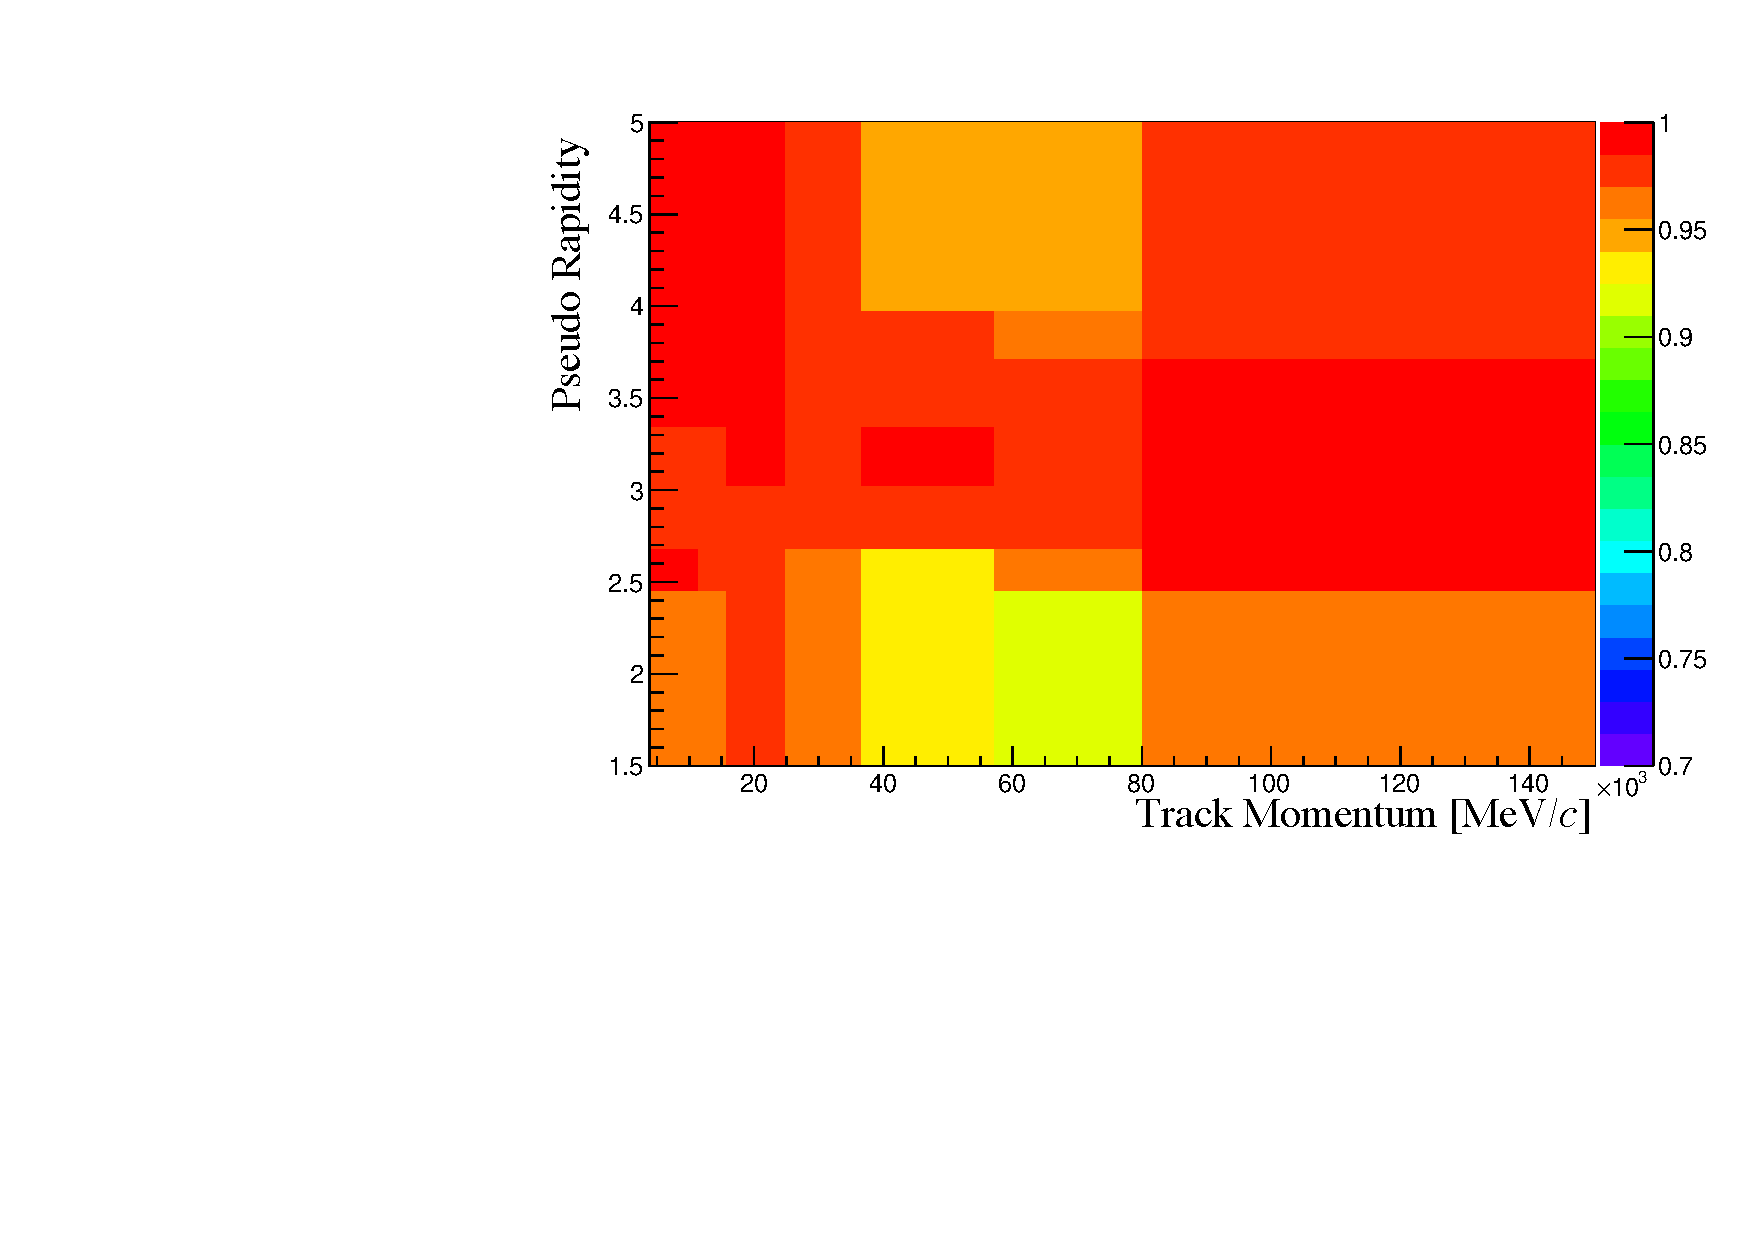
\includegraphics[width=0.48\textwidth]{RKst/figs/pid_Pi.pdf}
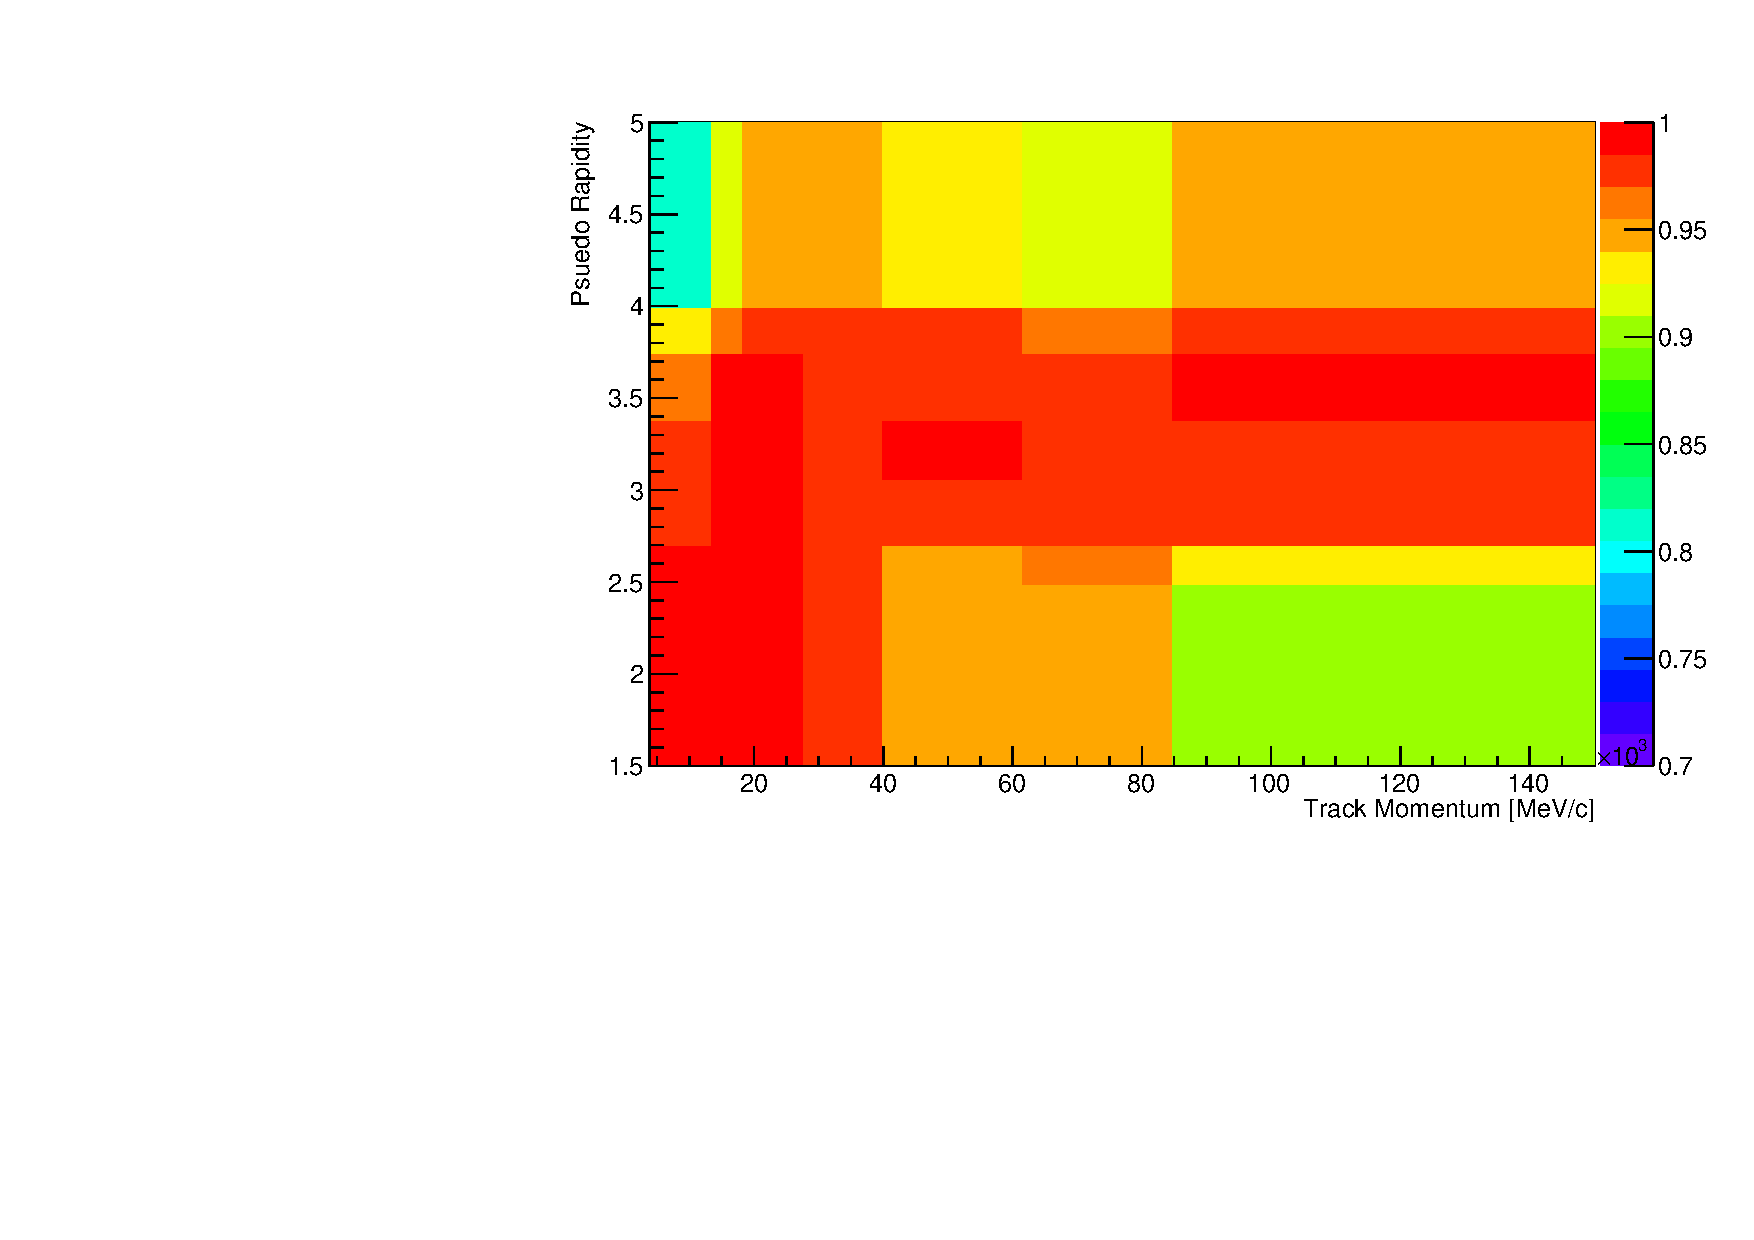
\includegraphics[width=0.48\textwidth]{RKst/figs/pid_K.pdf}
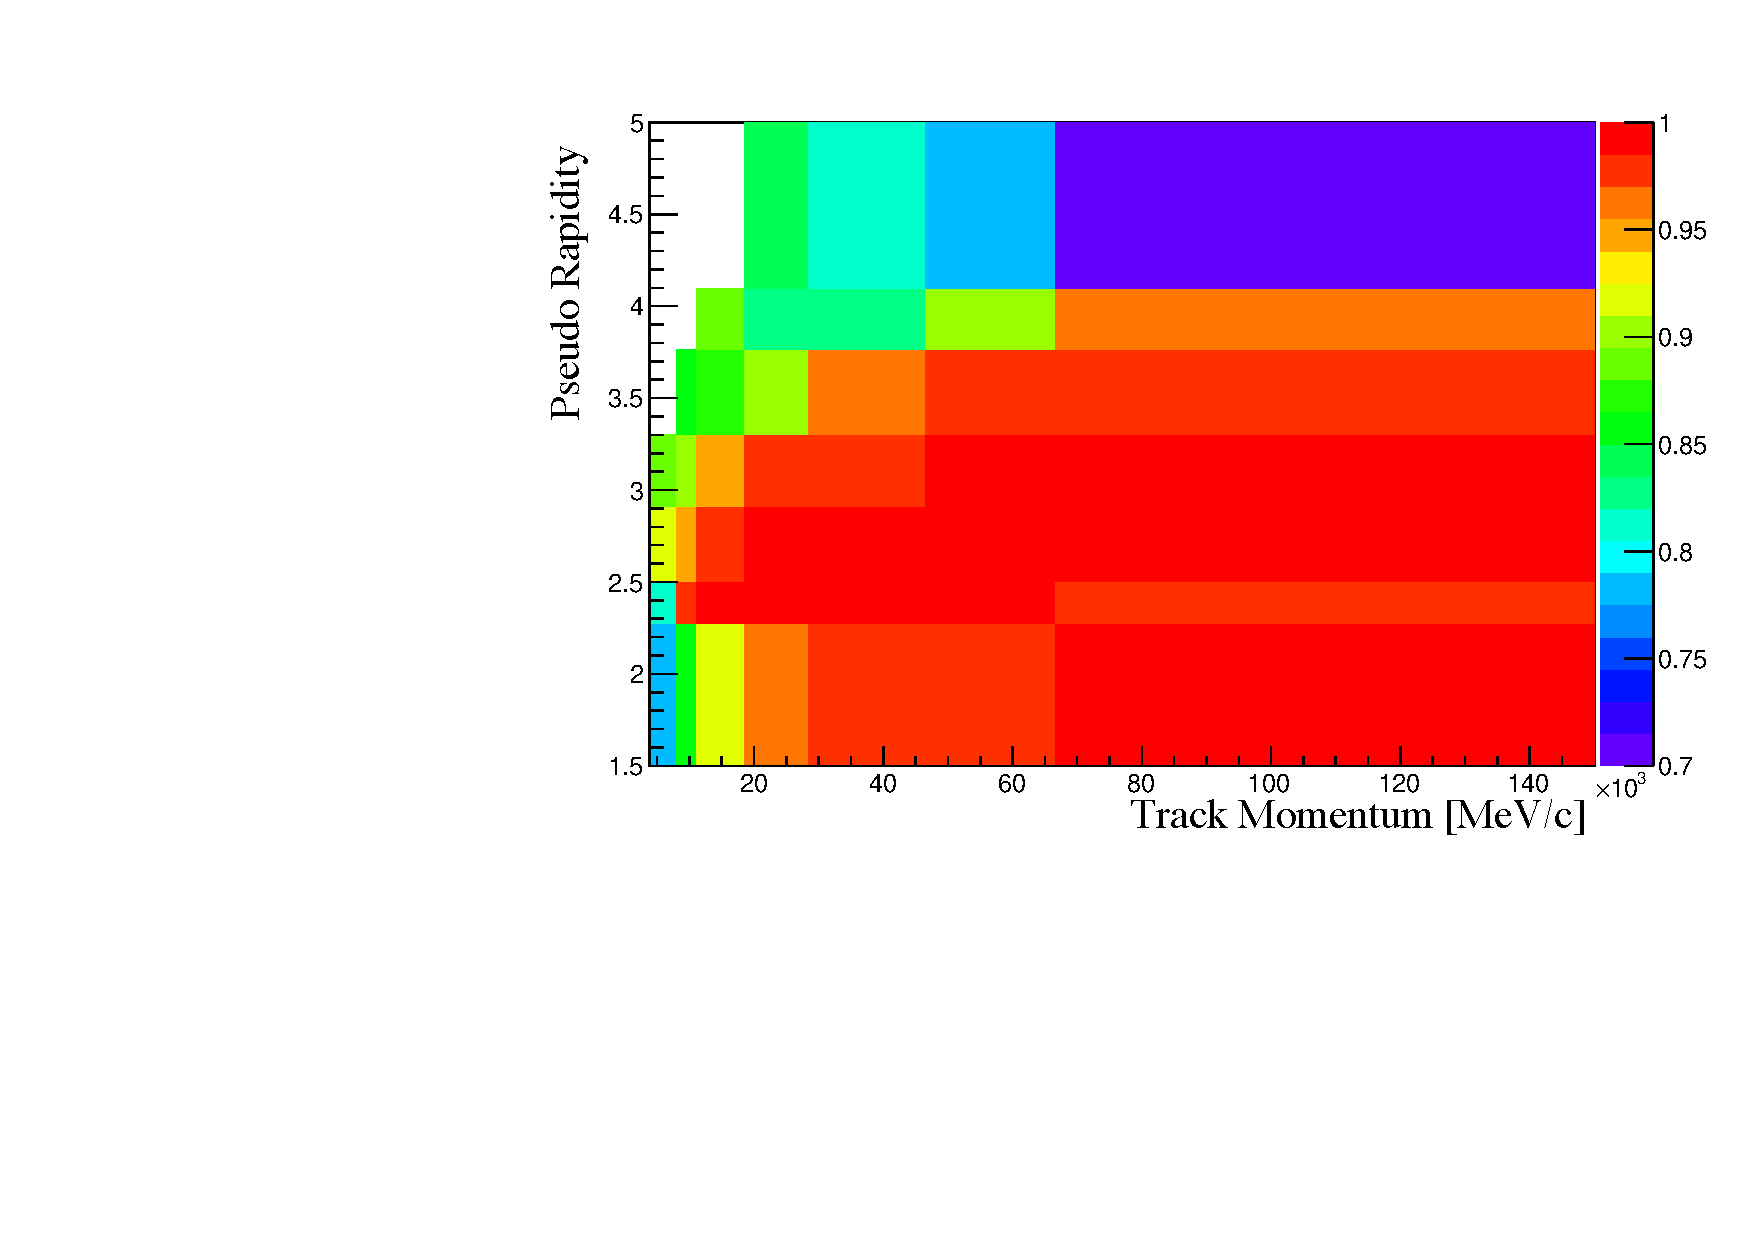
\includegraphics[width=0.48\textwidth]{RKst/figs/pid_Mu.pdf}
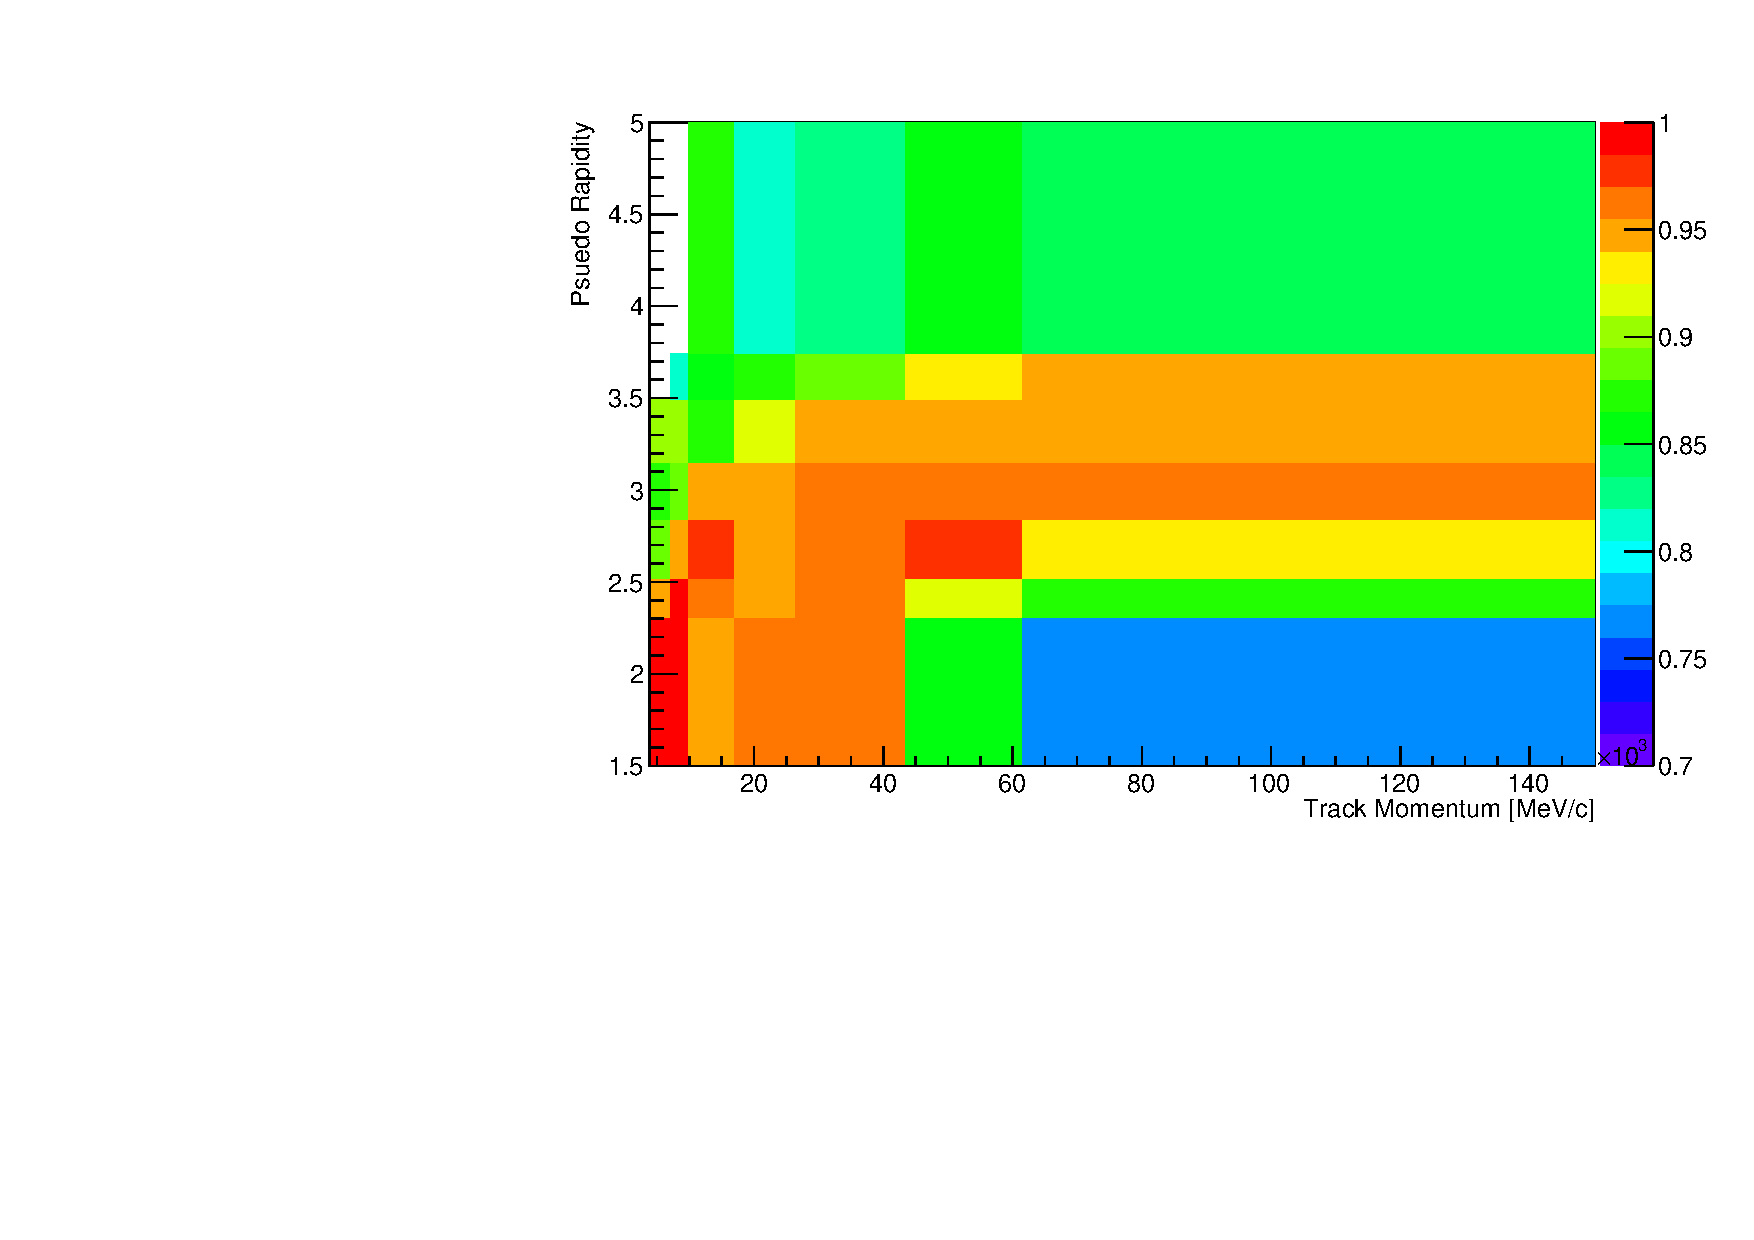
\includegraphics[width=0.48\textwidth]{RKst/figs/pid_e.pdf}
\caption{Performance tables obtained with data-driven methods
for pions (top left), kaons (top right), muons (bottom left) and electrons (bottom right).}
\label{fig:pid_perf_hist}
\end{figure}


\section{Trigger efficiency}
\label{sec:RKst_trigger_eff}

While the muon channels the trigger efficiency is calculated using simulated events,
for the electron channels a combinatin of simulation and data-driven methods is used.
The effciency of the software stage, Hlt, is always obtained from simulation,
while the efficiency of the hardware stage, L0, is obtained using a data-driven method
as described in the next section.
For both muon and electronc channels it is possible to use the resonant sample to crosscheck
the efficiency obtained using the simulation as explained in Sec.~\ref{sec:tistos}.

\subsection{Electron channels}

For the electron channels data is fitted separately in three trigger categories: L0Electron, L0Hadon and L0TIS.
Therefore we need to extract the efficiency separately for each category.

While the Hlt (1 and 2) efficiency is still computed using simulated events,
the L0Electron and L0Hadron efficiencies cannot be modelled with the Monte Carlo.
The discrepancy between data and simulation is mainly due to the ageing of the 
calorimeters, on which the decision of these triggers relies. The ageing is not simulated
in the Monte Carlo and affects the L0 trigger efficiency which, therefore, must
be calibrated using data driven-methods. Tables of efficiencies are obtained
applying the TIS-TOS method to a calibration sample.

For each trigger category these tables contain efficiency as a function of
\pt of the considered particle and are given for different calorimeter regions
as these have different properties (e.g. cell size) due to the different position
with respect to the beam line. Regions considered are inner and outer HCAL, and inner, middle and outer ECAL.
Figure~\ref{sec:L0eff_tables} shows data-driven efficiencies for the L0Electron trigger
in the three ECAL regions.
%
\begin{figure}[h!]
\centering
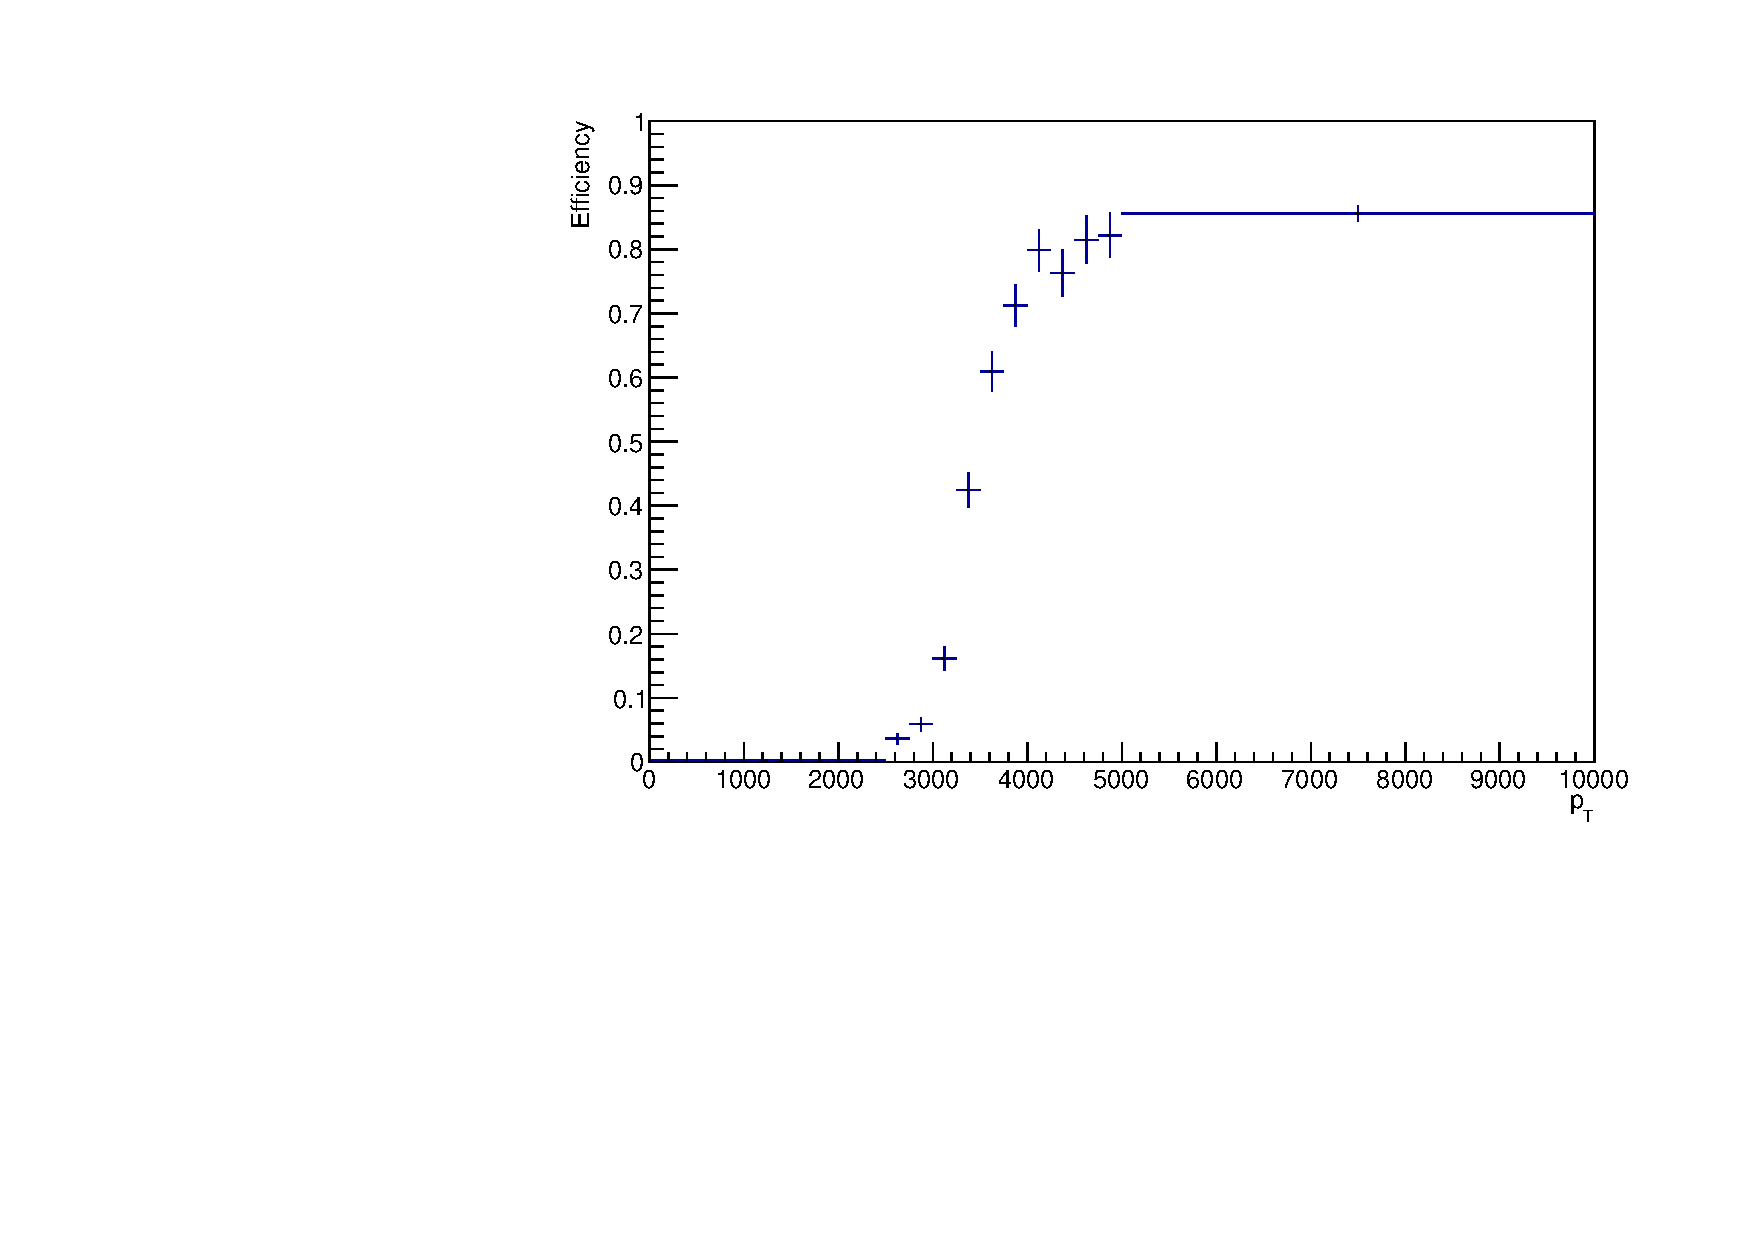
\includegraphics[width=0.49\textwidth]{RKst/figs/l0plots/l0E_Inner.pdf}
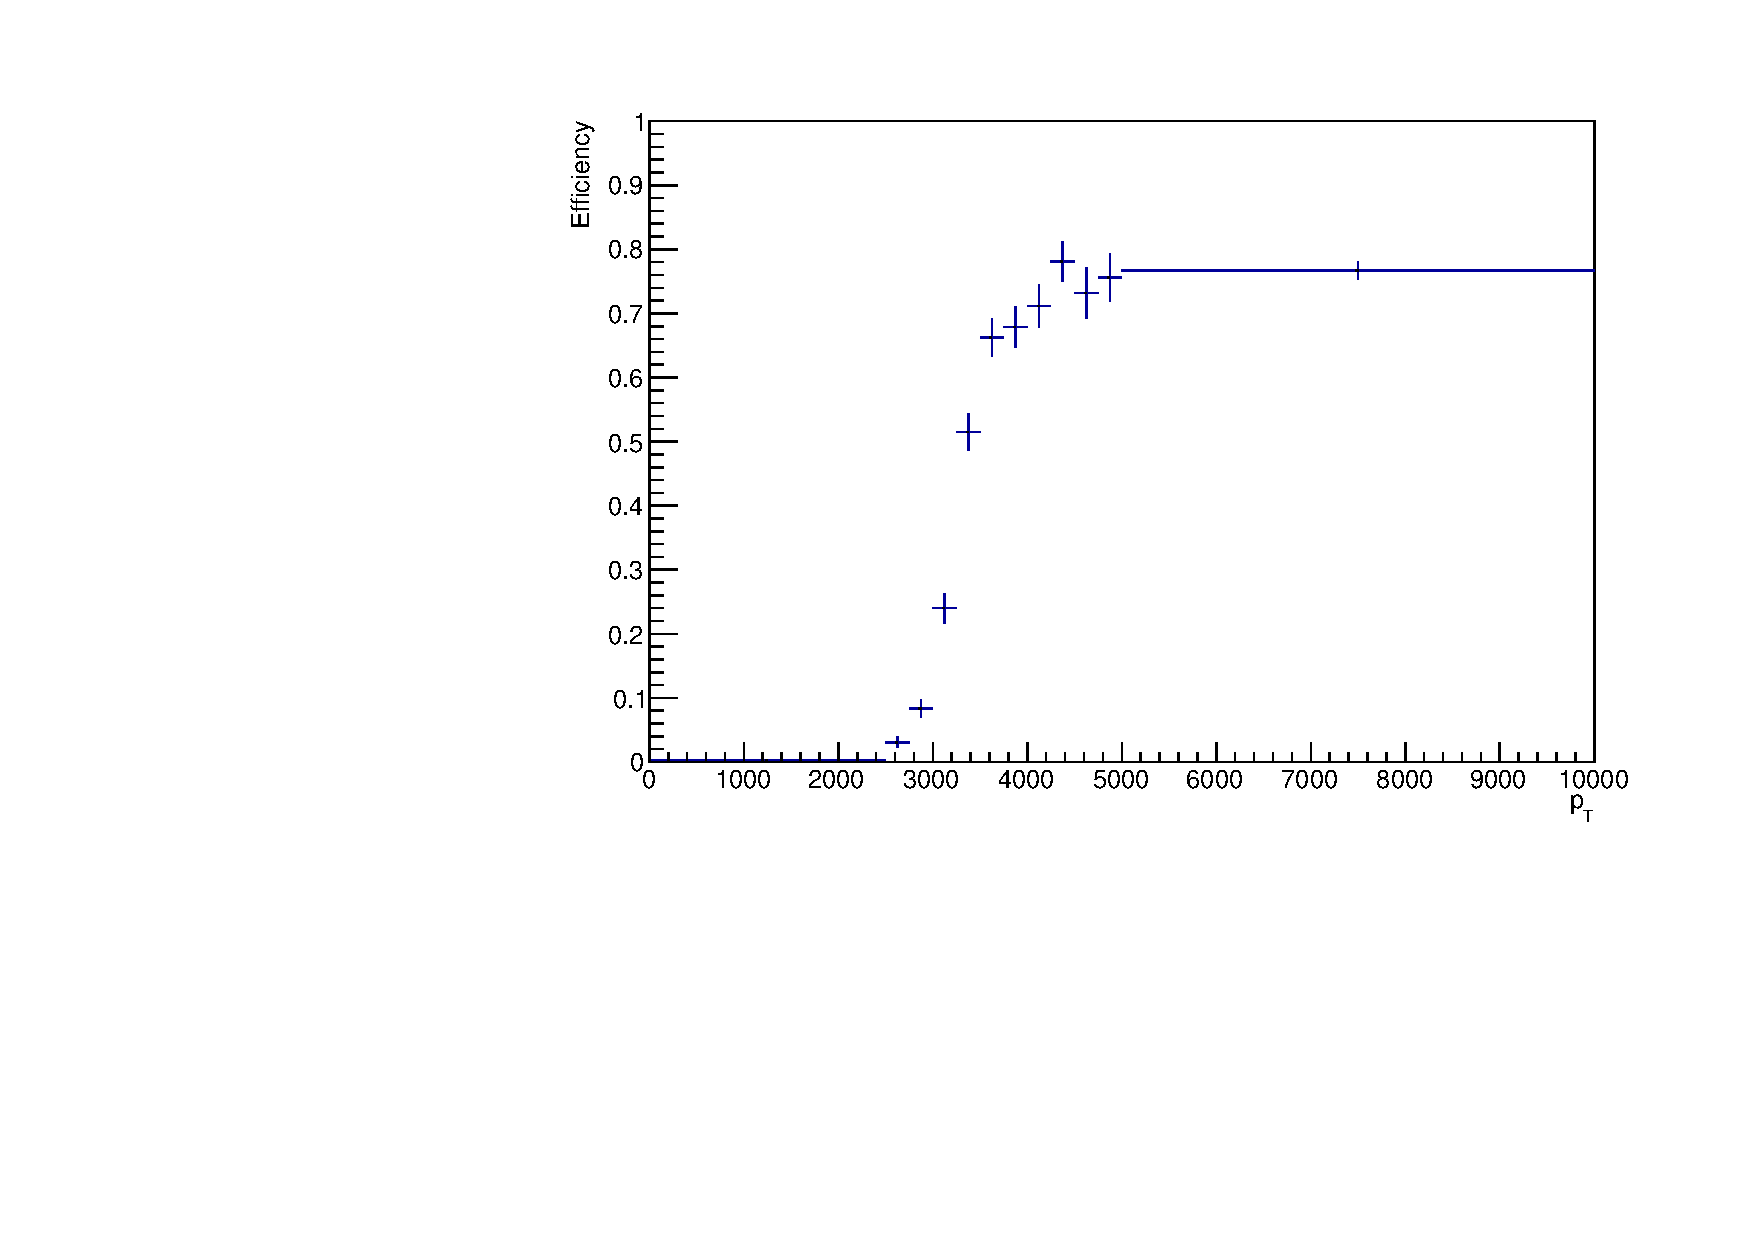
\includegraphics[width=0.49\textwidth]{RKst/figs/l0plots/l0E_Middle.pdf}
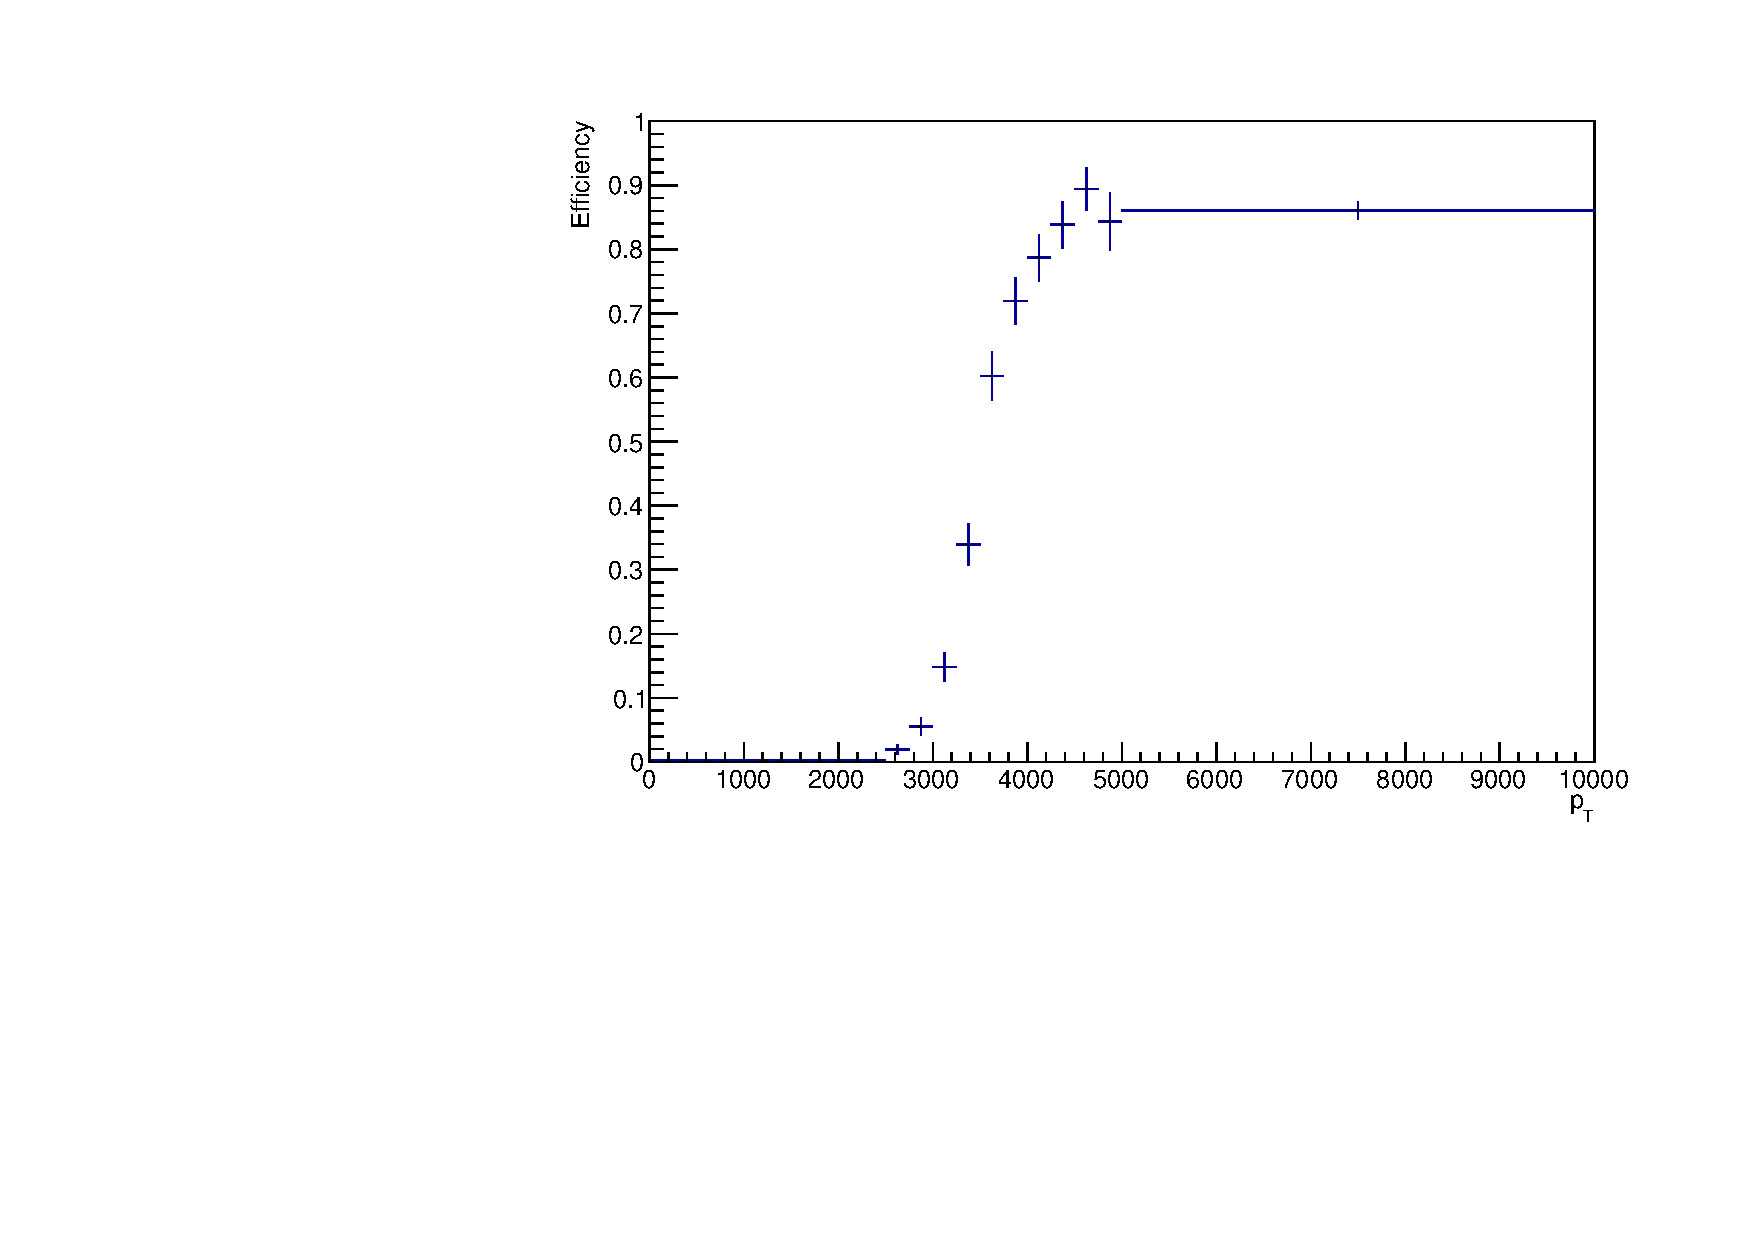
\includegraphics[width=0.49\textwidth]{RKst/figs/l0plots/l0E_Outer.pdf}
\caption{Data-driven L0Electron trigger efficiencies as a function of the transverse momentum
of the electrons for the three ECAL regions.}
\label{sec:L0eff_tables}
\end{figure}

The probability of L0Electron trigger is calculated for each event as $P_{L0E} = \varepsilon(e^+) + \varepsilon(e^-) - \varepsilon(e^+)\varepsilon(e^-)$.
Similarly, the L0Hadron trigger probability is $P_{L0H} = \varepsilon(\pi) + \varepsilon(K) - \varepsilon(\pi)\varepsilon(K)$.
For L0TIS a probability $P_{L0I} = (1-P_{L0E})\cdot(1-P_{L0H})$ is calculated.
Note that the probability of TIS trigger is defined to be independent of the signal and therefore must
be the same in the rare and resonant channels and cancel in their ratio.

Then event by event efficiencies for the three trigger categories are defined to be exclusive in the following way:
%
\begin{itemize}
\item L0E: $\varepsilon^{L0E} = P_{L0E}$, namely the probability that at least one electron triggered;
\item L0H: $\varepsilon^{L0H} = P_{L0H}\cdot(1 - P_{L0E})$, namely the probability that at least one hadron triggered but none of the electrons;
\item L0I: $\varepsilon^{L0I} = (1-P_{L0H})\cdot(1 - P_{L0E})$, namely the probability that neither the hadrons or the electrons in the event triggered. Note that in this case $\varepsilon^{L0I} $ does not correspond to the efficiency of L0TIS trigger.
\end{itemize}
%
%The total efficiency for each category is then found by using the kinematic distribution from MC events,
%weighted for PID efficiencies, SPD and \Bz $p_T$ as described in \ref{sec:MCweighting}.
As in the PID case, the total efficiency is found averaging over all events of a simulated sample:
%
\begin{equation}
\varepsilon^{\rm trg} = \frac{1}{N} \sum_i^N \varepsilon^{\rm trg}(\pt^i)
\end{equation}
\noindent
where trg" is a label indicating the trigger category under consideration.

\subsection{TISTOS cross-check}
\label{sec:tistos}

The efficiency obtained using the simulation
is crosschecked on resonant data using the TISTOS method already described in Sec.~\ref{sec:Lb_trigger_eff}.
%
%In LHCb triggered events can fall in two categories: events triggered by a track which is part
%of the candidate decay of interest, Trigger On Signal (TOS), or by other tracks in the event,
%Trigger Independent of Signal (TIS). All trigger lines used for this analysis are required to be TOS.
%The TIS and TOS samples are not exclusive but independent. Therefore the efficiency for TOS
%trigger can be obtained by data by the following formula:
%\begin{equation}
%\varepsilon_{TOS} = \frac{TOS \mbox{ and } TIS}{TIS}
%\end{equation}
%
For this purpose the logical $and$ of \verb!L0Global_TIS!, \verb!Hlt1Phys_TIS! and \verb!Hlt2Phys_TIS!
are used as control sample (TIS). As data also contains non negligible amounts of background
the \verb!DecayTreeFitter! tool is used to constrain the \jpsi mass to its known value
and a narrow interval around the peak, dominated by the signal, is selected.
Finally, to remove residual background in the data sample the $_{s}\mathcal{P}lot$ method is used. 
Results are shown in Tab.~\ref{tab:tistos}, where the
efficiency obtained using the TISTOS method is compared between data and simulation.
Efficiencies obtained on simulation and data are found to be in agreement for the muon channel
while they show deviations in the electron channels. Especially for the L0I category,
for which the procedure explained in Sec.~\ref{sec:trigee} does not ensure a correct calibration,
a significant discrepancy is found. The table also reports a correction factor
obtained according to the formula
\begin{equation}
f = 1 + \frac{\varepsilon_{date}^{TISTOS} - \varepsilon_{MC}^{TISTOS}}{\varepsilon_{MC}^{TISTOS}}
\end{equation}
which is used to correct the resonant yields as described in Sec.~\ref{sec:jpsicheck}.

No correction is applied for the extraction of the $R_{\Kstarz}$ ratio because
these discrepancies do not affect the ratio between the rare and resonant samples.
To check this the efficiency obtained using the TISTOS method
is plot as a function of the kinematic quantity relevant for each trigger category:
the maximum \pt of the electrons for L0E, the maximum \pt of $p$ and $\pi$ for L0H,
and the maximum \pt of all the final particles for L0I. Results are shown in Fig.~\ref{fig:tistos_vs_pt}.
The rare and resonant simulated samples are used to find the average efficiency in the two cases.
This corresponds to making an average of the efficiency weighted by the kinematical distributions
in the two samples. This procedure is applied using the efficiency obtained using the TISTOS method
and data and simulation and the two are compared. The ratios between the relative efficiencies, 
$(\varepsilon^{data}_{\ell\ell} / \varepsilon^{data}_{\jpsi}) / (\varepsilon^{sim}_{\ell\ell} / \varepsilon^{sim}_{\jpsi})$,
are found to be ??? for L0E, ??? for L0H and ??? for L0I, which are all compatible with one. 

\begin{table}[hb!]
\begin{center}
 \caption{Trigger efficiencies obtained using the TISTOS method on
 simulated and real $\decay{\Bz}{\Kstarz(\jpsi\to\ell\ell)}$ decays.}
\begin{tabular}{|c|c|c|c|}
\hline
 Sample 							&  MC  			& Data 		& Correction factor		\\ \hline
$ J/\psi \rightarrow \mu\mu$ 		& $ 0.797  \pm  0.002 $ & $ 0.803  \pm  0.004 $  &  1.0073  \\
$J/\psi \rightarrow ee$ L0E 	& $ 0.268  \pm  0.002 $ & $ 0.255  \pm  0.004 $  &  0.9536   \\
$J/\psi \rightarrow ee$ L0H 	& $ 0.028  \pm  0.001 $ & $ 0.026  \pm  0.002 $  &  0.9269   \\
$J/\psi \rightarrow ee$ L0I 	& $ 0.017  \pm  0.001 $ & $ 0.011  \pm  0.001 $  &  0.6760   \\
\hline 
\end{tabular}
\label{tab:tistos}
\end{center}
\end{table}

\begin{figure}[h!]
\centering
%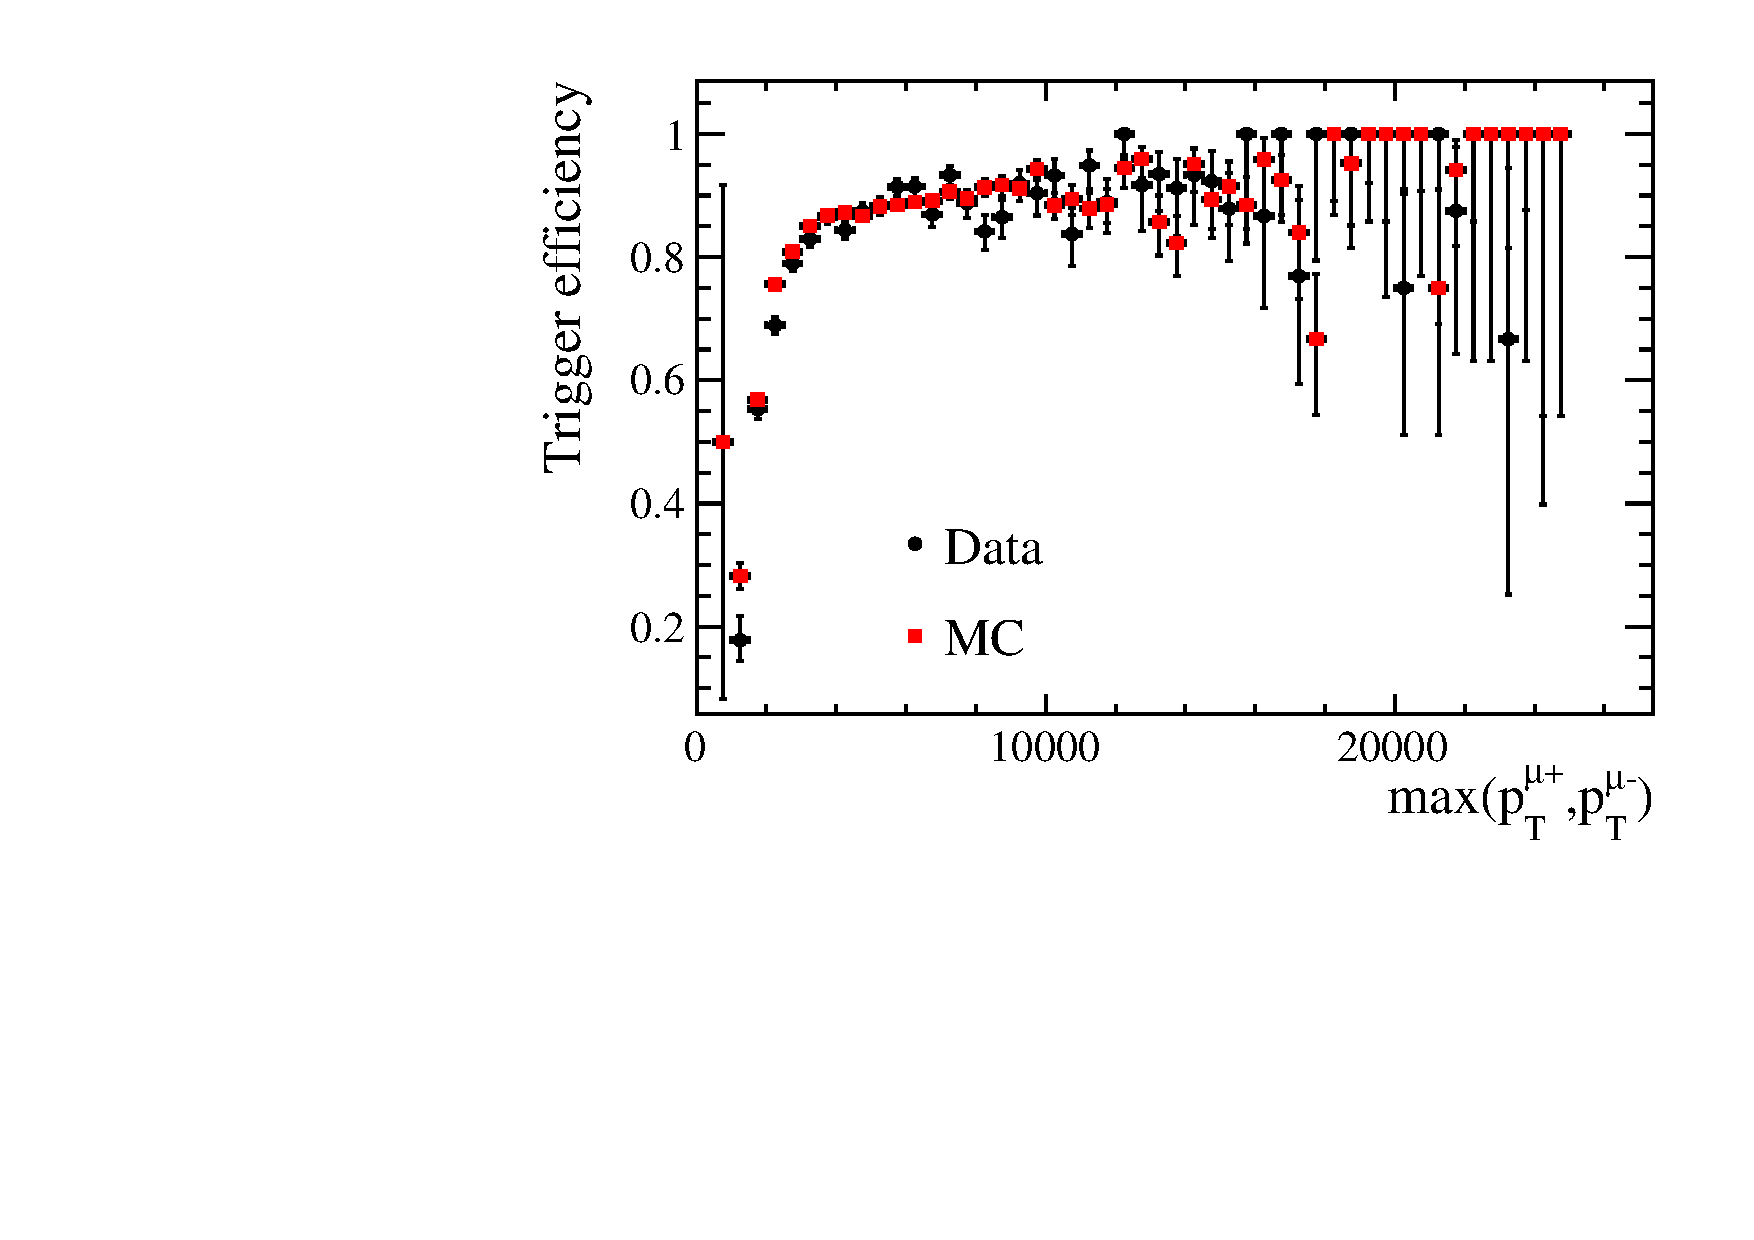
\includegraphics[width=0.48\textwidth]{figs/TisTos_vs_maxPTLL_MM.pdf}
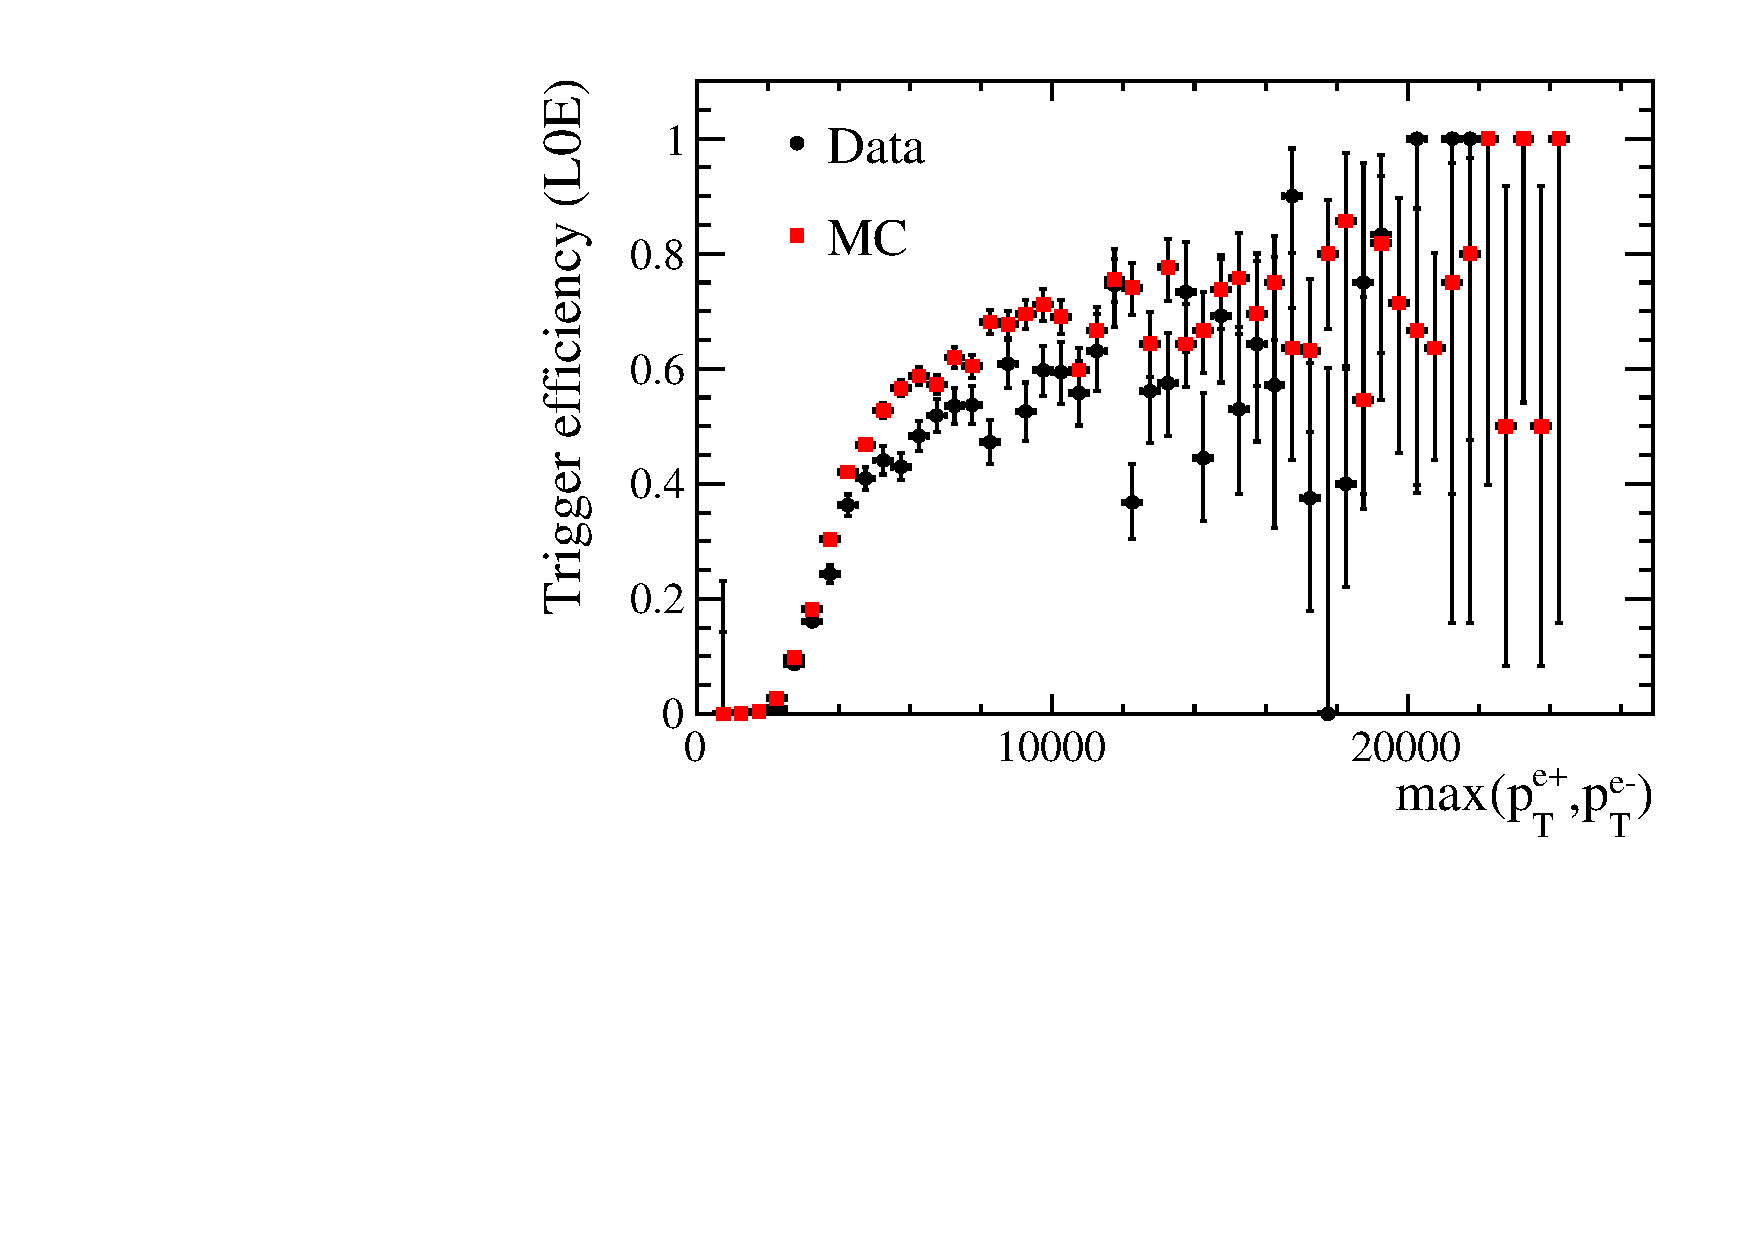
\includegraphics[width=0.48\textwidth]{RKst/figs/TisTos_vs_maxPTLL_L0E.pdf}
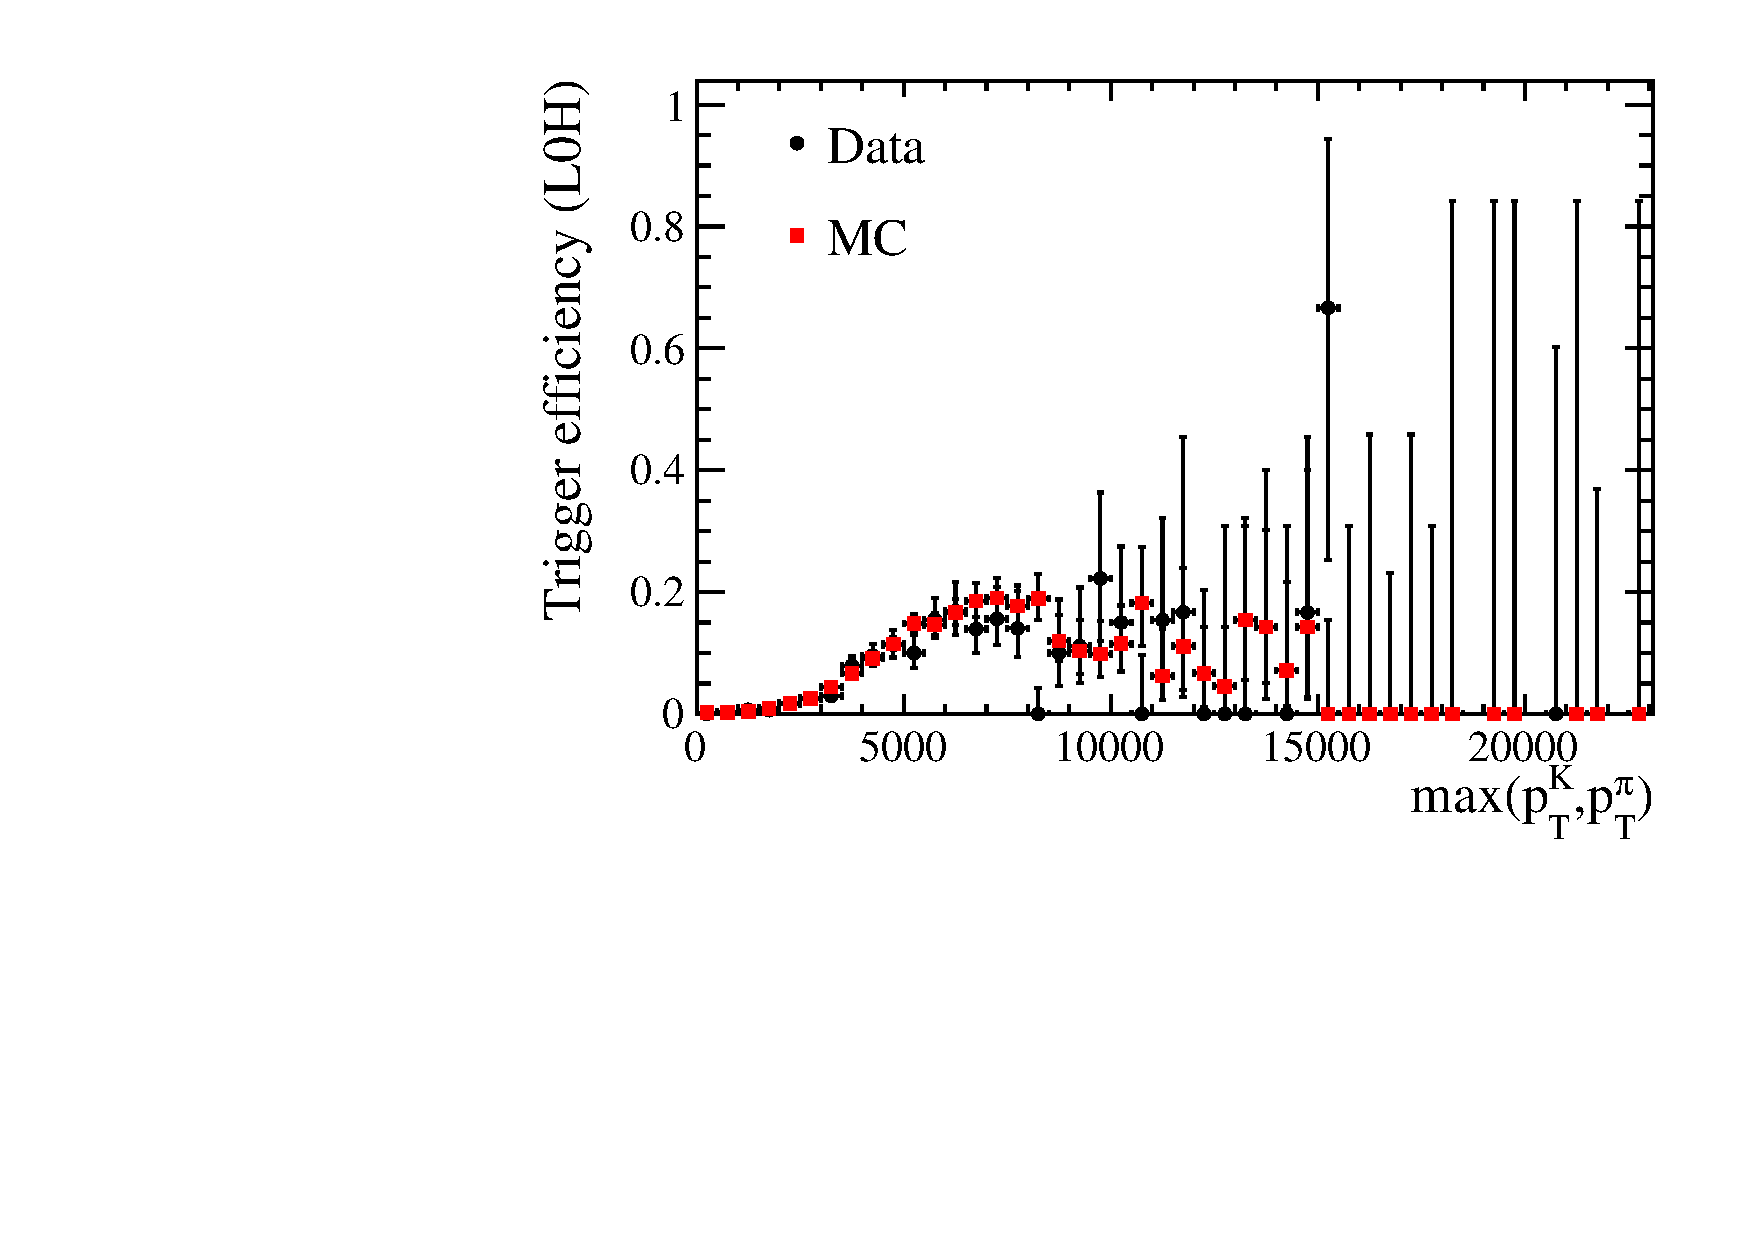
\includegraphics[width=0.48\textwidth]{RKst/figs/TisTos_vs_maxPTHH_L0H.pdf}
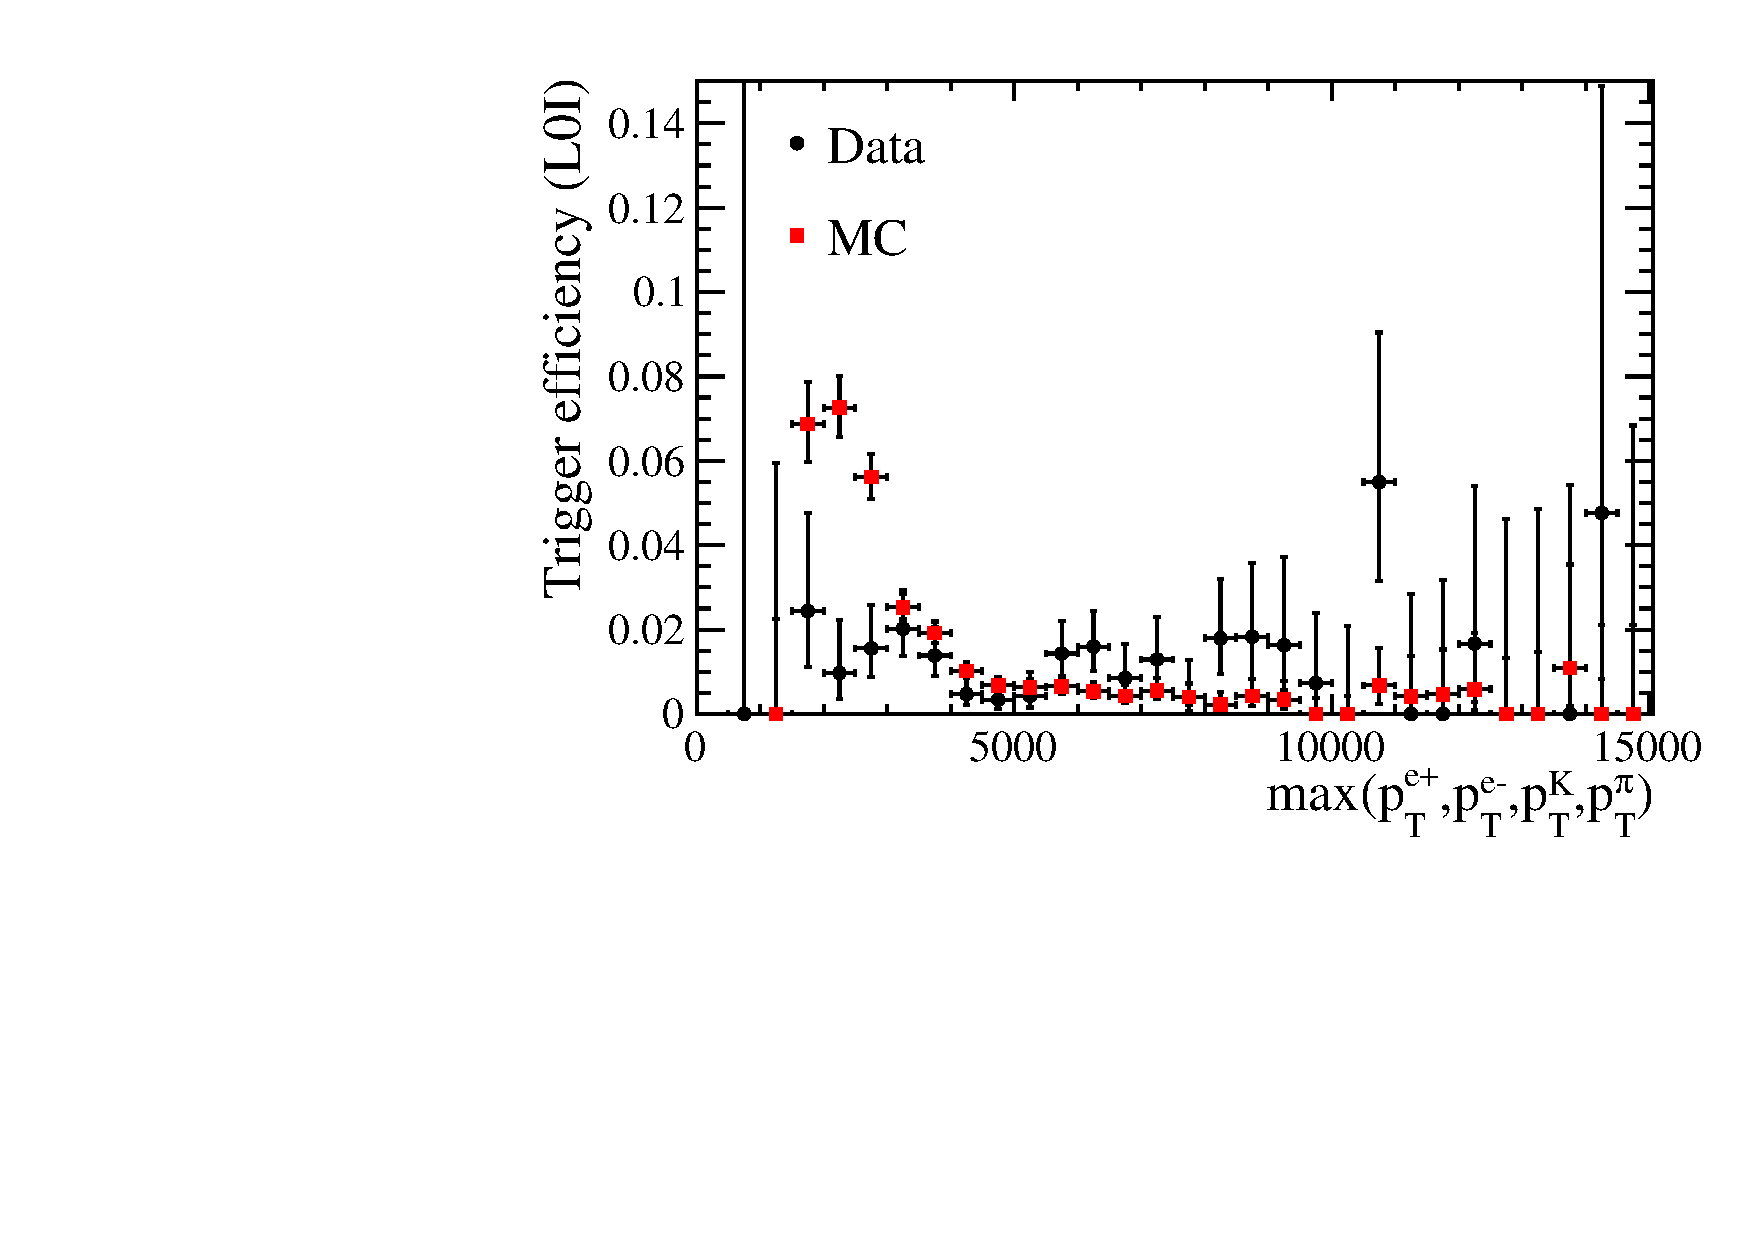
\includegraphics[width=0.48\textwidth]{RKst/figs/TisTos_vs_maxPT_L0I.pdf}
\caption{Trigger efficiency obtained applying the TISTOS method on $\Bz\to\jpsi\Kstar$ candiates
as a function of the maximum \pt of the electrons for the L0E category (top left), the maximum \pt
of $p$ and $\pi$ for L0H (top right) and the maximumm \pt of all the final particles for L0I (bottom).}
\label{fig:tistos_vs_pt}
\end{figure}


\section{Neural Networks efficiency}
\label{sec:Rkst_mva_eff}

The NN efficiency is again evaluated from fully weighted Monte Carlo samples. 
For the electron channels it is obtained separately for each trigger category.
%, because the yield is extracted independently for each of the three trigger categories
%and therefore these have to be independently corrected.

In order to cross check that this efficiency component is extracted correctly
one can compare the efficiency obtained using $\decay{\Bz}{\Kstarz(\jpsi\to\ll)}$ events
and rare $\decay{\Bz}{\Kstarz \ll}$ events in the same \qsq region selected
for the resonant case. The ratio between the two should be close to 1 with
small deviations due the fact that the bin width is finite and the events are distributed
differently inside the bin. This ratio is found to be $ 0.997  \pm  0.004 $ for the
$\mu\mu$ channels and on average $0.981  \pm  0.005$ for the $ee$ channels.
Values for the electron channels show a small deviation from one due to the very large
\qsq interval used to select the resonant channel ([6,11]~\gevgevcccc).

%\begin{table}[h!]
%\begin{tabular}{|c|c|c|c|c|}
%\hline Comp 			&  $\mu\mu$  				& \multicolumn {3}{c|}{$ee$}  \\ \hline
%				&   &  L0E 	& L0H 	& L0I \\ \hline
%rec  & $ 1.0104  \pm  0.0095 $ & \multicolumn{3}{c|}{$ 1.1040  \pm  0.0034 $} \\ 
%\hline
%trg  & $ 1.0113  \pm  0.0055 $ & $ 0.9752  \pm  0.0063 $ & $ 1.0078  \pm  0.0248 $ & $ 0.9766  \pm  0.0113 $ \\ 
%mva  & $ 0.9969  \pm  0.0039 $ & $ 0.9771  \pm  0.0023 $ & $ 0.9794  \pm  0.0019 $ & $ 0.9856  \pm  0.0057 $ \\ 
%\hline
%\end{tabular}
%\caption{Ratio $\varepsilon^{\ell\ell} / \varepsilon^{\jpsi}$ where the efficiency for the
%rare channel is calculated in the same \qsq range used to select the resonant channel.}
%\label{tab:mva_in_jpsibin}
%\end{table}


\clearpage








